\documentclass[cn]{elegantbook}
\usepackage[square,numbers,sort&compress]{natbib}
\newcommand{\upcite}[1]{\textsuperscript{\textsuperscript{\cite{#1}}}}

% title info
\title{模式识别文献综述}
\subtitle{基于深度学习的图像语义分割算法}
% bio info
\author{罗雁天}
\institute{清华大学电子系}
\version{2018310742}
\date{\today}
\logo{logo.png}
\cover{cover.jpg}

\begin{document}

\maketitle
\tableofcontents

\mainmatter
\hypersetup{pageanchor=true}
% add preface chapter here if needed
\chapter*{摘要}
在计算机视觉领域,图像分割指的是将数字图像细分为多个图像子区域(像素的集合)(也被称作超像素) 的过程。图像分割的目的是简化或改变图像的表示形式,使得图像更容易理解和分析。图像分割通常用于定位图像中的物体和边界(线,曲线等)。更精确的,图像分割是对图像中的每个像素加标签的一个过程,这一过程使得具有相同标签的像素具有某种共同视觉特性。

简单来说,图像分割可以看做是像素级别的分类,其在医疗领域、自动驾驶等方面有着重要的应用,在目前的算法研究中,图像分类可以分为语义分割、实例分割和全景分割。

本文主要从图像语义分割的方向进行调研,介绍了近几年来基于深度学习的图像语义分割算法,并且对这些算法进行对比与总结,最后提出了对图像分割未来方向的展望。

~\\

\noindent\textbf{关键字:图像语义分割;深度学习;全卷积网络;条件随机场}

\chapter*{Abstract}
In the field of computer vision, image segmentation refers to the process of subdividing a digital image into multiple image sub-regions (a collection of pixels) (also referred to as superpixels). The purpose of image segmentation is to simplify or change the representation of the image, making the image easier to understand and analyze. Image segmentation is often used to locate objects and boundaries (lines, curves, etc.) in an image. More precisely, image segmentation is a process of tagging each pixel in an image, which results in pixels with the same tag having some common visual characteristics.

In short, image segmentation can be regarded as a pixel-level classification, which has important applications in the medical field and automatic driving. In the current algorithm research, image classification can be divided into semantic segmentation, instance segmentation and panoptic segmentation.

This paper mainly investigates the direction of image semantic segmentation, introduces the image semantic segmentation algorithm based on deep learning in recent years, and compares and summarizes these algorithms. Finally, it puts forward the prospect of the future direction of image segmentation.

~\\

\noindent\textbf{Key Words: Image Semantic Segmentation; Deep Learning; Fully Convolutional Networks; Conditional Random Field}

\chapter{引言}
图像分割(Segmentation)指的是将数字图像细分为多个图像子区域(像素的集合)(也被称作超像素)的过程。图像分割的目的是简化或改变图像的表示形式,使得图像更容易理解和分析。图像分割通常用于定位图像中的物体和边界(线,曲线等)。更精确的,图像分割是对图像中的每个像素加标签的一个过程,这一过程使得具有相同标签的像素具有某种共同视觉特性。

图像分割又可以分为图像语义分割(Semantic Segmentation)与实例分割(Instance Segmentation)。语义分割是在像素级别上的分类,属于同一类的像素都要被归为一类,因此语义分割是从像素级别来理解图像的。而实例分割不但要进行像素级别的分类,还需在具体的类别基础上区别开不同的实例。比如说图像有多个人甲、乙、丙,那边他们的语义分割结果都是人,而实例分割结果却是不同的对象。

图像分割在实际应用中非常广泛,在医学影像中来用来进行肿瘤和其他病理的定位、组织体积的测量、计算机引导的手术等,在卫星图像中定位物体,用于人脸识别、指纹识别,近几年在自动驾驶领域图像分割也起着至关重要的作用。

\section{评价指标}
在图像分割领域主要有如下4个评价指标:
\begin{itemize}
	\item pixel accuracy (Acc): 像素准确率;
	\item mean pixel accuracy of different categories (mAcc): 类平均像素准确率;
	\item mean Intersection-over-Union of different categories (mIoU): 类平均识别准确度;
	\item frequency-weighted IoU (fwIoU): 频率加权的识别准确度。
\end{itemize}

其中IoU(Intersection-over-Union)表示预测位置与真实位置之间的重叠程度,IoU越高,预测的位置越准确。图\ref{IoU}表示了IoU的几何意义。

\begin{figure}
	\centering
	\begin{minipage}[t]{0.45\textwidth}
		\centering
		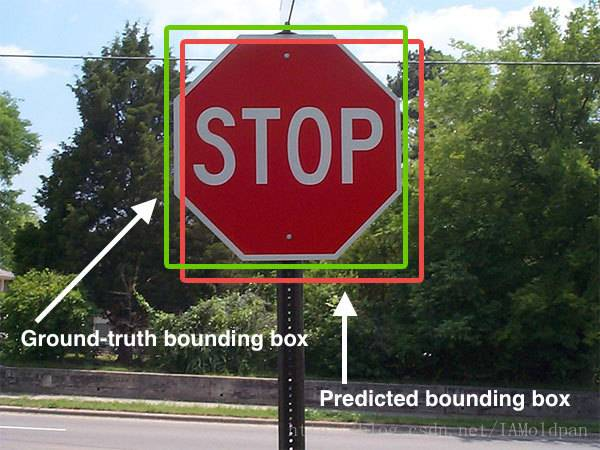
\includegraphics[width=4cm]{images/IoU1.jpg}
	\end{minipage}
	\begin{minipage}[t]{0.45\textwidth}
		\centering
		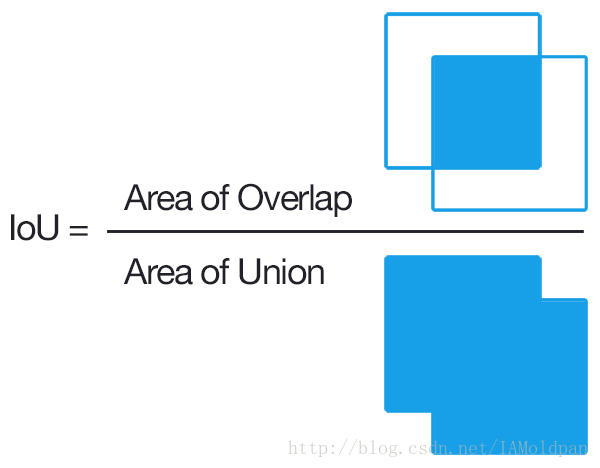
\includegraphics[width=4cm]{images/IoU2.png}
	\end{minipage}
	\caption{\label{IoU}IoU表示含义示意图}
\end{figure}

四个指标的计算方式如式\ref{eval}所示:
\begin{definition}{计算方式}{eval1}
	\begin{equation}
	\label{eval}
	\begin{aligned}
	Acc &= \sum_{i}\frac{n_{ii}}{s} \\
	mAcc &= \frac{1}{n_C}\sum_{i}\frac{n_{ii}}{s_i} \\
	mIoU &= \frac{1}{n_C}\sum_{i}\frac{n_{ii}}{s_i+\sum_{j}n_{ji}-n_{ii}} \\
	fwIoU &= \frac{1}{s}\sum_{i}s_i\frac{n_{ii}}{s_i+\sum_{j}n_{ji}-n_{ii}}
	\end{aligned}
	\end{equation}
\end{definition}

\section{数据集}
图像分割常用的数据集包括PASCAL VOC\upcite{everingham2015pascal}、MS COCO\upcite{2014arXiv1405.0312L}等,包含深度信息图像的数据集有NYUv2\upcite{silberman2012indoor}等。

\begin{itemize}
	\item PASCAL VOC(The PASCAL Visual Object Classification)是目标检测、分类、图像分割领域一个有名的数据集。从2005年到2012年,共举办了8个不同的挑战赛。用于图像分割的VOC2012数据集提供原图以及图像语义分割和图像实例分割两种png图(如图\ref{voc}所示),共分为20类,包括背景为21类,分别如下:
	\begin{itemize}
		\item[-] Person: person;
		\item[-] Animal: bird, cat, cow, dog, horse, sheep;
		\item[-] Vehicle: aeroplane, bicycle, boat, bus, car, motorbike, train;
		\item[-] Indoor: bottle, chair, dining table, potted plant, sofa, tv/monitor.
	\end{itemize}
    \begin{figure}[!h]
    	\centering
    	\begin{minipage}[t]{0.32\textwidth}
    		\centering
    		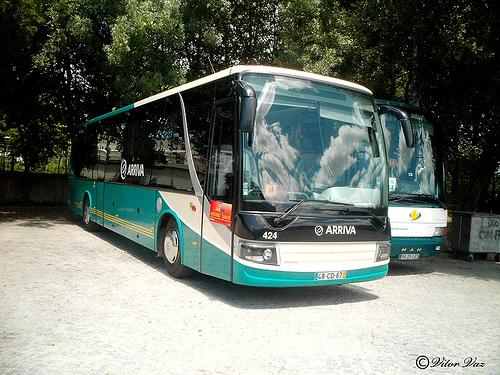
\includegraphics[width=\textwidth]{images/voc1}
    	\end{minipage}
    	\begin{minipage}[t]{0.32\textwidth}
    		\centering
    		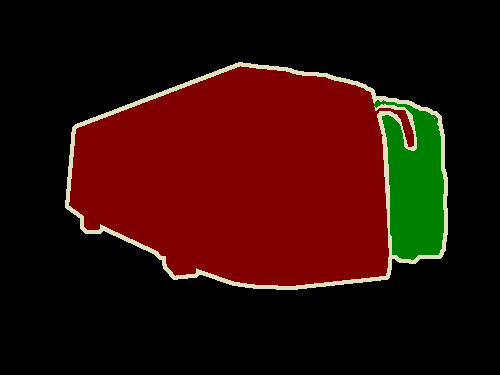
\includegraphics[width=\textwidth]{images/voc1_object.png}
    	\end{minipage}
    	\begin{minipage}[t]{0.32\textwidth}
    		\centering
    		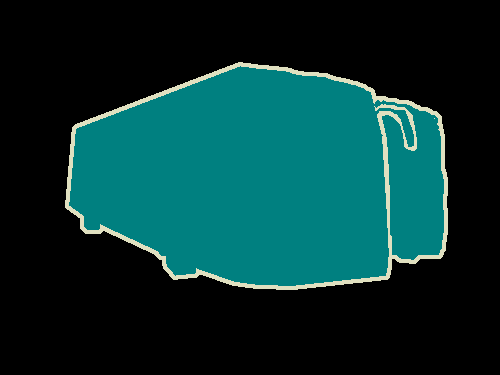
\includegraphics[width=\textwidth]{images/voc1_class.png}
    	\end{minipage}
    	\caption{\label{voc}PASCAL VOC图像分割数据集示例(左图:原始图像;中图:实例分割的标签图;右图:语义分割的标签图)}
    \end{figure}

	\item MS COCO(Common Objects in COntext)是微软建立的数据集。这个数据集也用于多种竞赛:图像标题生成、目标检测、关键点检测和图像分割。图像包括91类目标,328000影像和2500000个label。图\ref{coco}展示了MS COCO举办的各个竞赛中数据集的示例。
	
	\begin{figure}[!h]
		\centering
		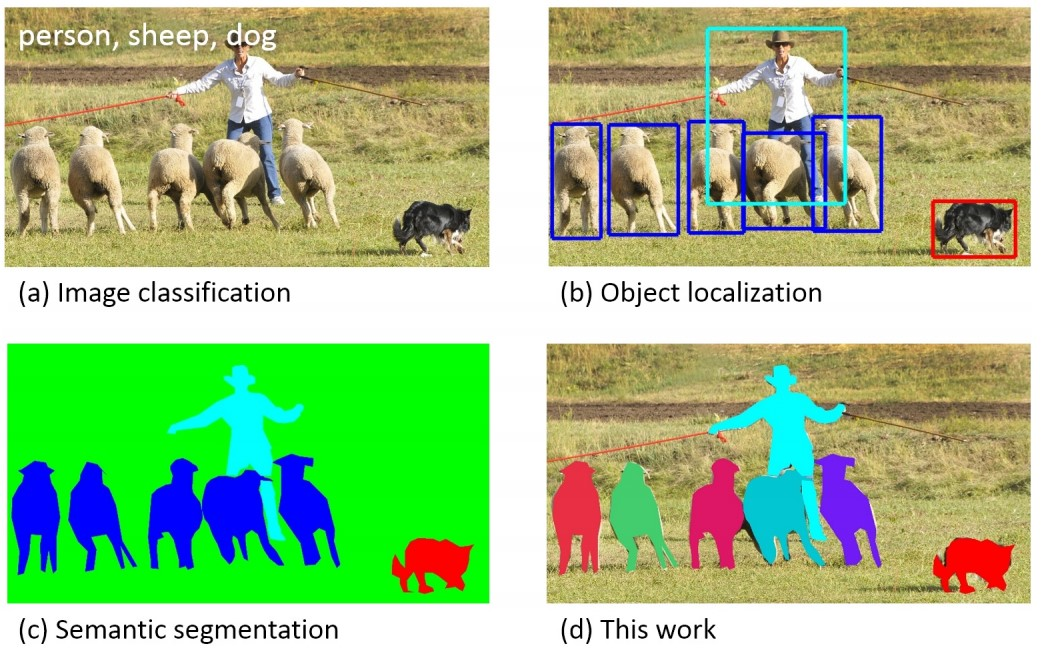
\includegraphics[width=\textwidth]{images/coco}
		\caption{\label{coco}MS COCO数据集多种图像任务示例}
	\end{figure}
	
	\item NYUv2数据集是使用Kinect采集的一系列包含深度信息的图像,包含如下几个部分:
	\begin{itemize}
		\item[-] 有标签的:视频数据的一个子集,伴随着密集多标签。此数据已被预处理以填补缺少的深度标签;
		\item[-] 原始数据集:利用Kinect测得的原始的RGB、Depth、加速度数据;
		\item[-] 工具箱:用于操作数据和标签的有用的工具;
		\item[-] 用于评估的训练和测试部分。
	\end{itemize}
    有标签的数据如图\ref{nyu1}所示。
    \begin{figure}[!h]
    	\centering
    	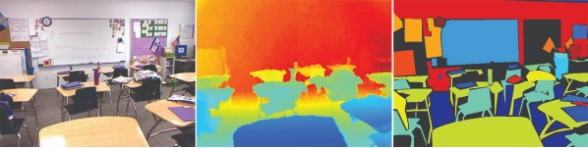
\includegraphics[width=\textwidth]{images/nyu1}
    	\caption{\label{nyu1}NYUv2有标签的数据集示例。(左图:Kinect相机输出的图像;中图:预处理深度信息;右图:添加一系列标签图)}
    \end{figure}
\end{itemize}

\section{综述结构}
本综述主要包含如下内容:
\begin{itemize}
	\item 第一章为引言部分,主要介绍了图像分割的评价指标以及图像分割方面的数据集;
	\item 第二章介绍了图像语义分割方向近几年来最经典的几种算法,并且在每一小节都与之前算法的实验结果进行了对比,从中我们可以直观的感受到图像分割实验效果的一步步提升;
	\item 第三章主要从2018年图像分割方向的论文出发,学习一下目前图像分割算法的研究方向;
	\item 第四章为对图像分割算法的总结以及对未来研究方向的展望。
\end{itemize}
\chapter{基于深度学习的经典图像语义分割算法}
在深度学习方法流行之前,TextonForest和基于随机森林分类器等语义分割方法是用得比较多的方法。不过在深度卷积网络流行之后,深度学习方法比传统方法提升了很多,所以这里就不详细讲传统方法了。最初的学习方法应用于图像分割就是Patch classification。Patch classification方法,顾名思义,图像是切成块喂给深度模型的,然后对像素进行分类。使用图像块的主要原因是因为全连接层需要固定大小的图像。由于在全卷积网络出现之后对语义分割的效果提升了很多,因此在此也不再详述Patch Classification的方法。

\section{全卷积网络(FCN)}
全卷积网络(Fully convolutional networks, FCN\upcite{long2015fully})于2015年被首次提出,并且获得了当年CVPR的best paper。相比于之前使用带全连接层的卷积神经网络进行图像分割,FCN主要涉及以下三个技术:
\begin{itemize}
	\item 卷积化(Convolutionalization);
	\item 上采样(Upsampling),也叫反卷积(Deconvoltion);
	\item 跳跃结构(Skip Architecture).
\end{itemize}

\subsection{卷积化}
FCN将传统CNN中的全连接层转化为一个个的卷积层。如图\ref{fcn}所示,上图为传统的CNN网络结构(AlexNet\cite{krizhevsky2012imagenet}),前5层是卷积层,第6层和第7层分别是一个长度为4096的全连接层,第8层是一个长度为1000的全连接层。在FCN中,将最后的三层全连接层全都替换为卷积层,卷积核大小分别为(4096,1,1), (4096,1,1), (1000,1,1)。

\begin{figure}[!h]
	\centering
	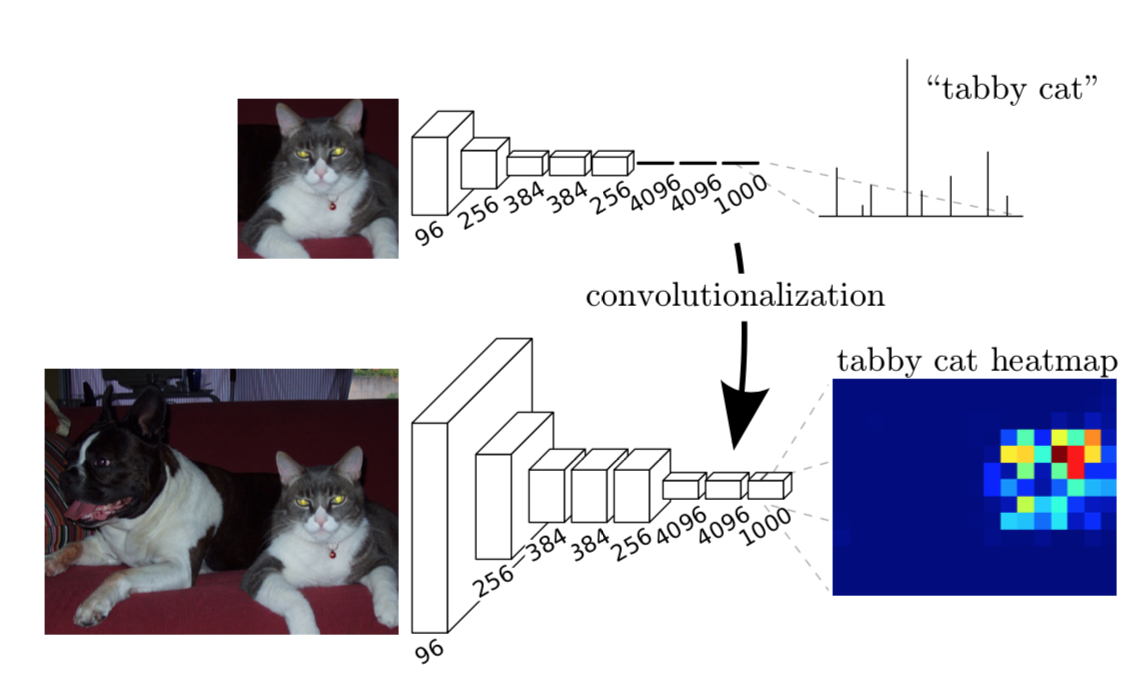
\includegraphics[width=\textwidth]{images/fcn}
	\caption{\label{fcn}FCN与传统CNN对比图}
\end{figure}

网络结构如图\ref{fcn1}所示,虚线上半部分为全卷积网络(蓝:卷积层,绿:max pooling),输入可为任意尺寸的图像,下半部分为反卷积(上采样)结构,最后输出与原图像大小相同,通道数为21(PASCAL VOC数据集20类物体类别+1类背景).

\begin{figure}[!h]
	\centering
	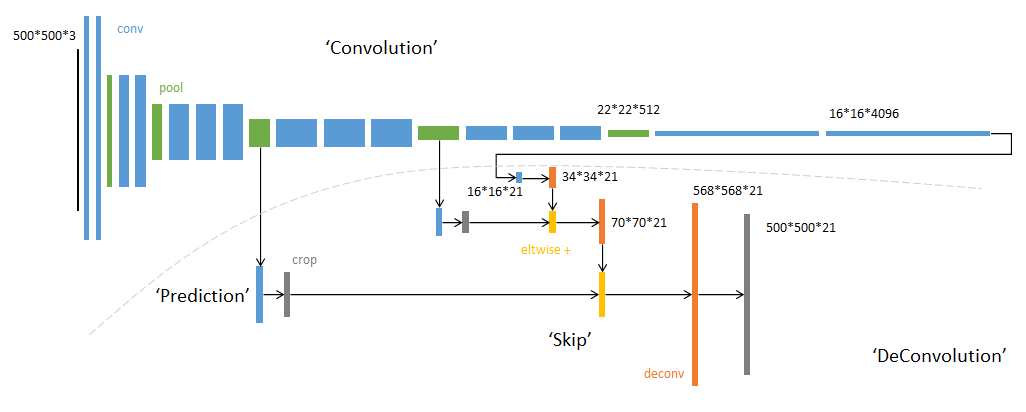
\includegraphics[width=\textwidth]{images/fcn1}
	\caption{\label{fcn1}FCN网络结构示意图}
\end{figure}

\subsection{反卷积}
经过全卷积网络之后得到的feature map相比于原图像要小,为了得到和原图像一样的feature map以便进行像素级的分类,FCN采用反卷积的方式将最后一层的feature map进行放大(图\ref{fcn1}中虚线以下橙色的部分)。

图\ref{deconv}展示了正常卷积与反卷积的对比图,左图展示的正常的no padding no strides情况下的卷积操作,可以看出,卷积之后feature map会变小,右图展示的是no padding no strides情况下的反卷积操作,可以看出反卷积之后feature map会增大。简单来看,反卷积其实可以看做先对feature map进行上采样增加像素,然后再进行卷积的过程,卷积的参数值通过训练得到。

\href{https://github.com/vdumoulin/conv_arithmetic}{https://github.com/vdumoulin/conv\_arithmetic}给出了各种类型卷积的动态图(正常卷积、反卷积以及之后要涉及的空洞卷积),可以通过动态图进一步认识各种卷积操作。论文\cite{dumoulin2016guide}给出了详细的数学公式以及卷积前后feature map大小的变化公式,可以更深一步的认识卷积。


\begin{figure}
	\centering
	\begin{minipage}[t]{0.45\textwidth}
		\centering
		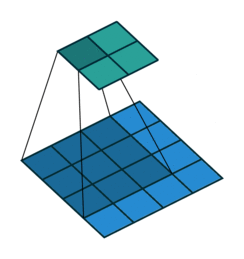
\includegraphics[width=\textwidth]{images/no_padding_no_strides-0.png}
	\end{minipage}
	\begin{minipage}[t]{0.45\textwidth}
		\centering
		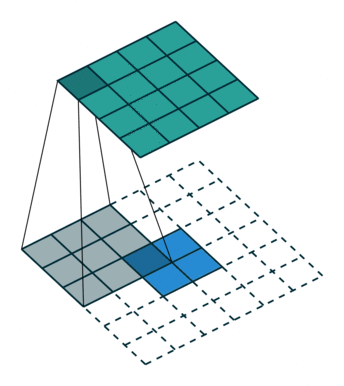
\includegraphics[width=\textwidth]{images/no_padding_no_strides_transposed-0.png}
	\end{minipage}
	\caption{\label{deconv}正常卷积与反卷积对比图}
\end{figure}

\subsection{跳跃结构}
如图\ref{skip}所示展示了FCN中跳跃结构示意图。从图中可以看出,对原图进行卷积conv1、pool1后图像缩小为1/2;对图像进行第二次卷积conv2、pool2后图像缩小为1/4;对图像进行第三次卷积conv3、pool3后图像缩小为1/8,此时保留pool3的featuremap;对图像进行第四次卷积conv4、pool4后图像缩小为1/16,此时保留pool4的featuremap;对图像进行第五次卷积conv5、pool5后图像缩小为1/32,然后把原来CNN操作过程中的全连接编程卷积操作的conv6、conv7,图像的featuremap的大小依然为原图的1/32,此时图像不再叫featuremap而是叫heatmap。其实直接使用前两种结构就已经可以得到结果了,这个上采样是通过反卷积(deconvolution)实现的,对第五层的输出(32倍放大)反卷积到原图大小。但是得到的结果还上不不够精确,一些细节无法恢复。于是将第四层的输出和第三层的输出也依次反卷积,分别需要16倍和8倍上采样,结果过也更精细一些了。这种做法的好处是兼顾了local和global信息。

\begin{figure}[ht]
	\centering
	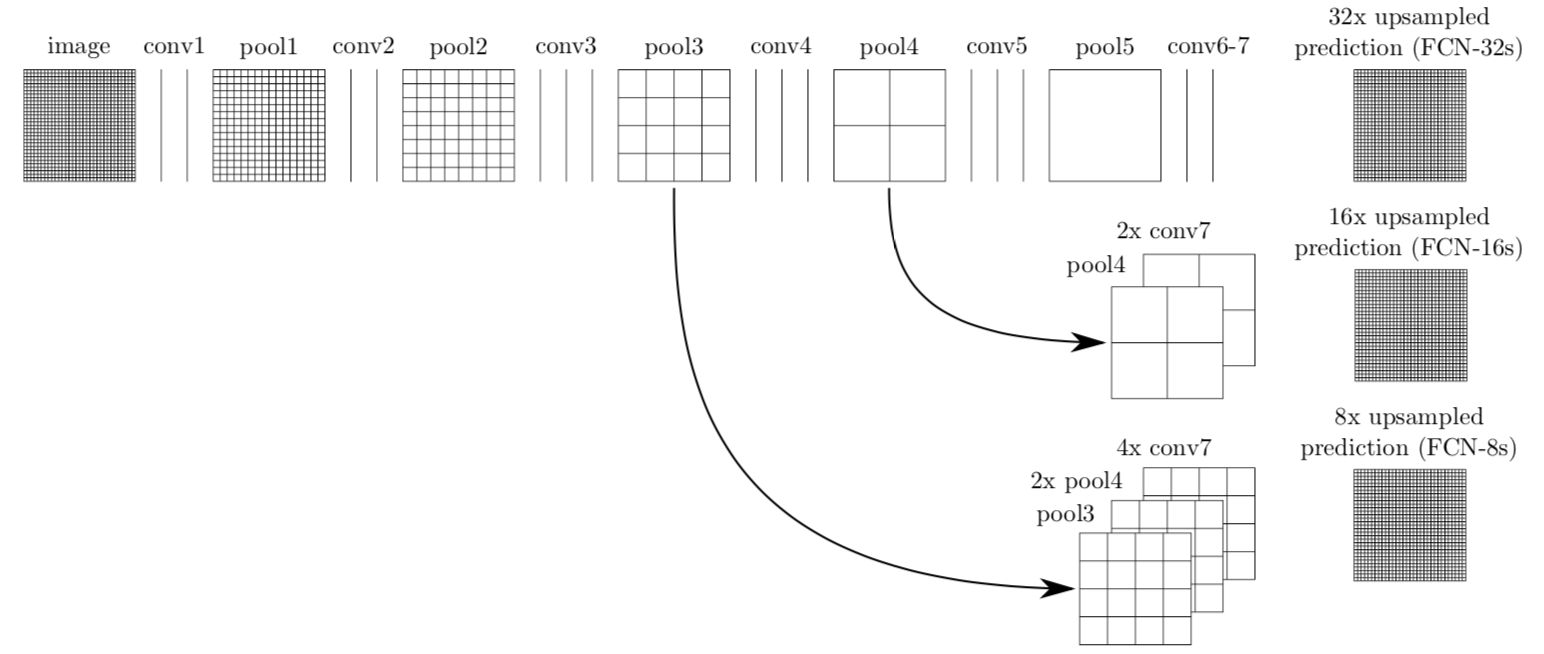
\includegraphics[width=\textwidth]{images/skip.png}
	\caption{\label{skip}跳跃结构示意图}
\end{figure}

\subsection{实验结果}
在此篇论文中,作者分别使用了一次反卷积、两次反卷积以及三次反卷积操作进行实验,并且使用修改过的VGG网络结构进行训练,最后在PASCAL VOC数据集上的性能指标如图\ref{fcnres}所示。由结果图中可以直观的看出,FCN的图像分割结果和ground truth相比已经有了较好的效果,但是边缘部分差距还是较大,在之后的几种算法中会有进一步的提升。

\begin{figure}[!h]
	\centering
	\begin{minipage}[t]{0.85\textwidth}
		\centering
		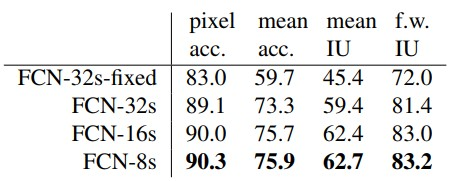
\includegraphics[width=\textwidth]{images/fcnres}
	\end{minipage}
	\begin{minipage}[t]{0.85\textwidth}
		\centering
		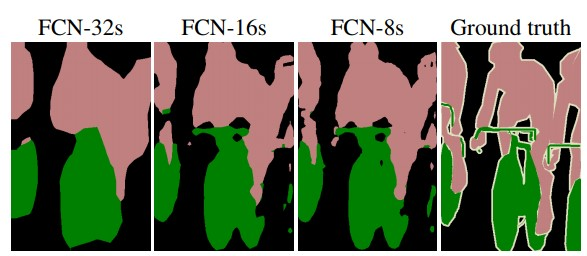
\includegraphics[width=\textwidth]{images/fcnres1}
	\end{minipage}
	\caption{\label{fcnres}实验结果性能指标与PASCAL VOC数据集上的实验效果图}
\end{figure}

\section{DeepLab}
从FCN的实验结果图中可以看出来,虽然分割的整体区域比较正确了,但是分割效果还是比较粗糙,细节不明显。DeepLab v1(文章\cite{chen2014semantic},发表于ICLR2015)使用Hole算法(Atrous Algorithm)和条件随机场(CRF)来进一步的提升分割效果,其算法结构图如图\ref{deeplabv1}所示。DeepLab v1收录于ICLR 2015,是DeepLab系列的第一篇文章,之后我们还会介绍该系列的后续文章。

\begin{figure}[!h]
	\centering
	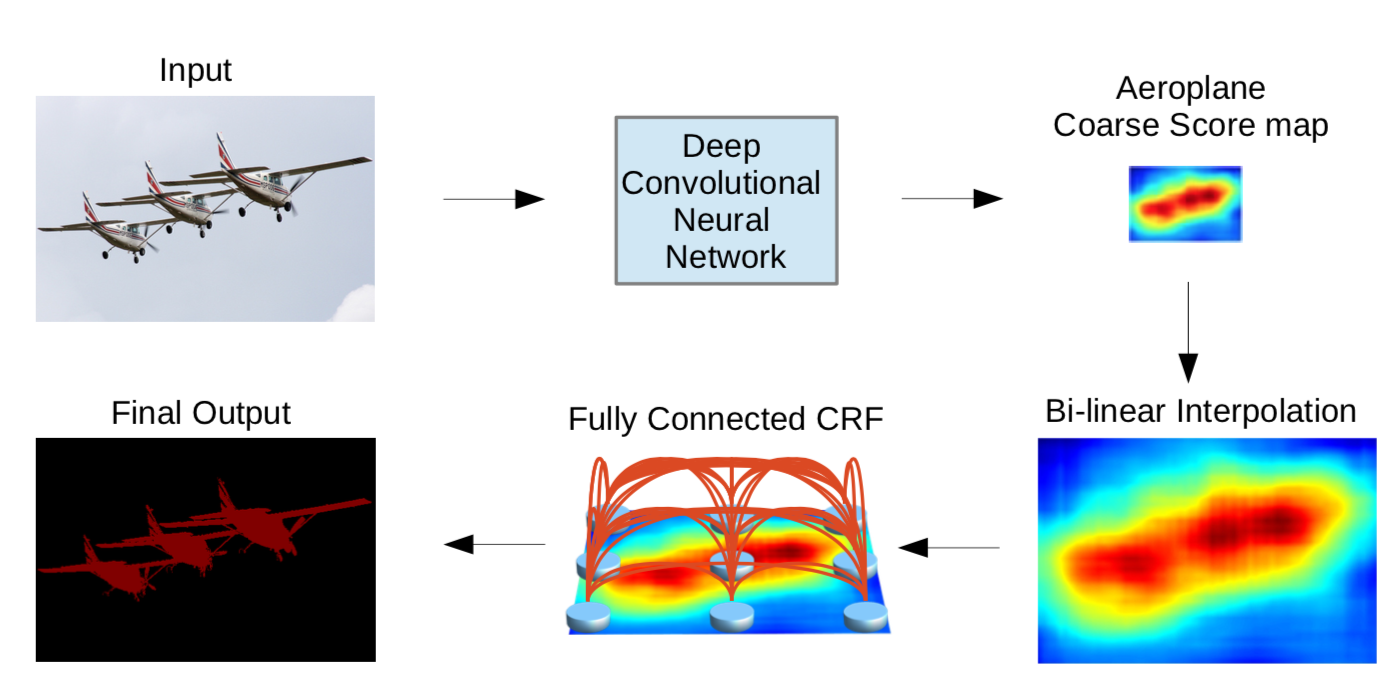
\includegraphics[width=\textwidth]{images/deeplabv1}
	\caption{\label{deeplabv1}DeepLab算法结构示意图}
\end{figure}

\subsection{Hole算法}
由于普通的卷积感受野较小,需要增加池化层来增加感受野,但是池化层又会损失信息,所以使用空洞卷积在不损失信息的情况下增加感受野的范围。

Hole算法又可以看做带孔(Hole)卷积,传统的卷积或者pooling中,一个filter中相邻的权重作用在feature map上的位置都是物理上连续的。而在Hole算法中,一个filter中相邻的权重不一定作用在feature map上的位置都是物理上连续的,而是跟hole size相关的。如图\ref{hole}所示表示的是卷积核大小kernel\_size=3,输入步长input\_stride(也就是hole size)=2,输出步长output\_stride=1的一维带孔卷积示意图。可以看出卷积核作用在输入feature map上的位置不是连续的。后续章节会有关于Hole算法的更详细的介绍,在此不再赘述。


\begin{figure}[!h]
	\centering
	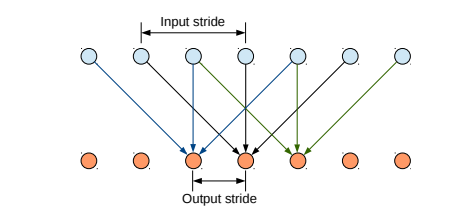
\includegraphics[width=\textwidth]{images/hole}
	\caption{\label{hole}Hole算法示意图}
\end{figure}

\subsection{条件随机场}
只使用全卷积网络能够预测到目标的大概位置但是位置比较模糊,论文\cite{krahenbuhl2011efficient}中提出的全连接条件随机场尝试找到图像像素之间的关系:相近且相似的像素大概率为同一标签,考虑像素的概率分配标签,通过迭代来细化分割的结果。

条件随机场服从吉布斯分布,如式(\ref{gibbs})所示,其中$E(X)$是$x$取某个值的能量,$Z(I)$是归一化的函数。
\begin{equation}
\label{gibbs}
P(X|I)=\frac{1}{Z(I)}\exp(-E(X|I))
\end{equation}

为了做图像分割,只需要后验概率最大,因此只需能量函数最小即可,因此条件随机场优化的目标函数便是能量函数$E(X)$(式(\ref{energy})).
\begin{equation}
\label{energy}
E(x)=\sum_i \psi_i(x_i)+\sum_{i,j} \psi_{i,j}(x_i,x_j)
\end{equation}

能量方程的第一项$\psi_i(x_i)$(式(\ref{unary}))称为一元势函数,用于衡量当像素点$i$的颜色值为$y_i$时,该像素点属于类别标签$x_i$的概率。在DeepLab中,此概率是通过CNN的输出得到的。
\begin{equation}
\label{unary}
\psi_i(x_i)=-\log(P(x_i))
\end{equation}

能量方程的第二项$\psi_{i,j}(x_i,x_j)$称之为成对势函数(pairwise),用于衡量两事件同时发生的概率$p(x_i,x_j)$,我们希望两个相邻的像素点,如果颜色值$y_i,y_j$非常接近,那么这两个像素点$x_i,x_j$属于同一个类别的概率应该比较大才对;反之如果颜色差异比较大,那么我们分割的结果从这两个像素点裂开的概率应该比较大才对。这一能量项正是为了让我们的分割结果尽量从图像边缘的地方裂开,也就是为了弥补之前FCN边缘的地方分割的不足,我们可以采用式(\ref{pairwise})来计算。
\begin{equation}
\label{pairwise}
\psi_{i,j}(x_i,x_j)=u(x_i,x_j)\sum_{m=1}^{M}w^mK_G^m(f_i,f_j)
\end{equation}
其中$K_G$是一个高斯核,用于度量像素点$i$和$j$的特征向量相似度的一个高斯权重项。特征向量$f_i$我们可以用$(x,y,R,G,B)$表示,也就是以像素点的像素值和坐标位置作为特征向量。然后$u(x_i,x_j)$表示两个标签之间的一个兼容性度量。通过最小化式(\ref{energy})的能量函数,我们就可以实现CRF隐变量$X$的推理。

图\ref{crf1}显示了DeepLab中使用CRF迭代来细化分割结果的示意图,从图中可以看出,使用CRF迭代可以使得分割的边缘效果逐渐增强。
\begin{figure}[!h]
	\centering
	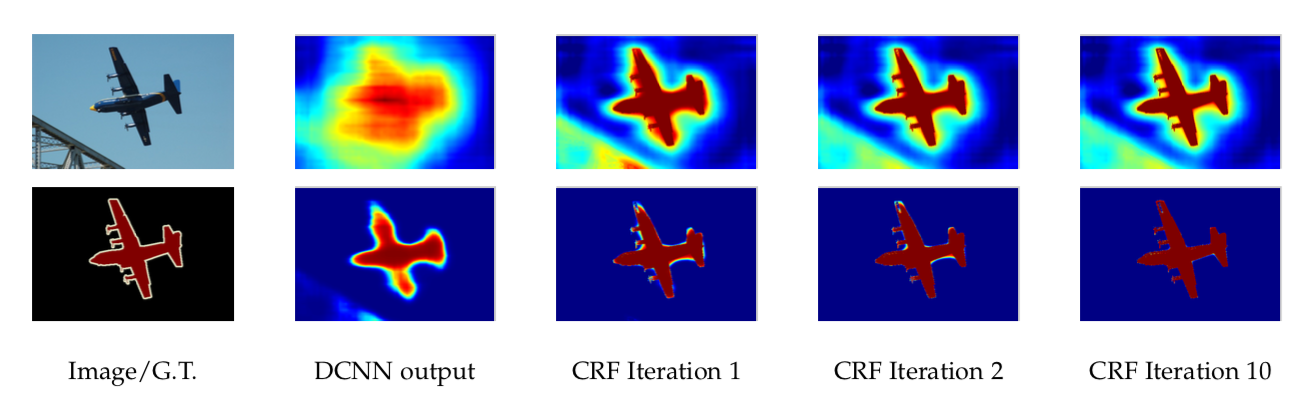
\includegraphics[width=\textwidth]{images/crf}
	\caption{\label{crf1}使用CRF细化分割效果。可以看出,随着迭代次数的增加,图像分割的效果逐渐增强}
\end{figure}

\subsection{实验结果}
DeepLab综合了之前出现的全卷积网络FCN,提出了带洞卷积,在此我们列出与FCN算法在PASCAL VOC数据集上实验效果对比如图\ref{deeplabvsfcn}所示。从图中可以看出,DeepLab在边缘部分的分割效果相比于FCN有了进一步的提升。

\begin{figure}[!h]
	\centering
	\begin{minipage}[t]{0.85\textwidth}
		\centering
		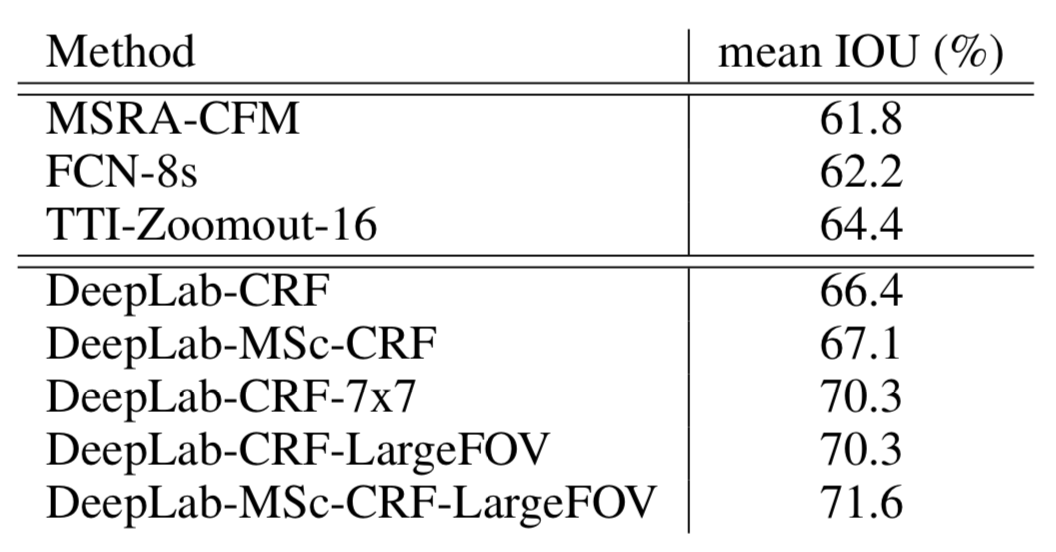
\includegraphics[width=\textwidth]{images/deeplabvsfcn1}
	\end{minipage}
	\begin{minipage}[t]{0.85\textwidth}
		\centering
		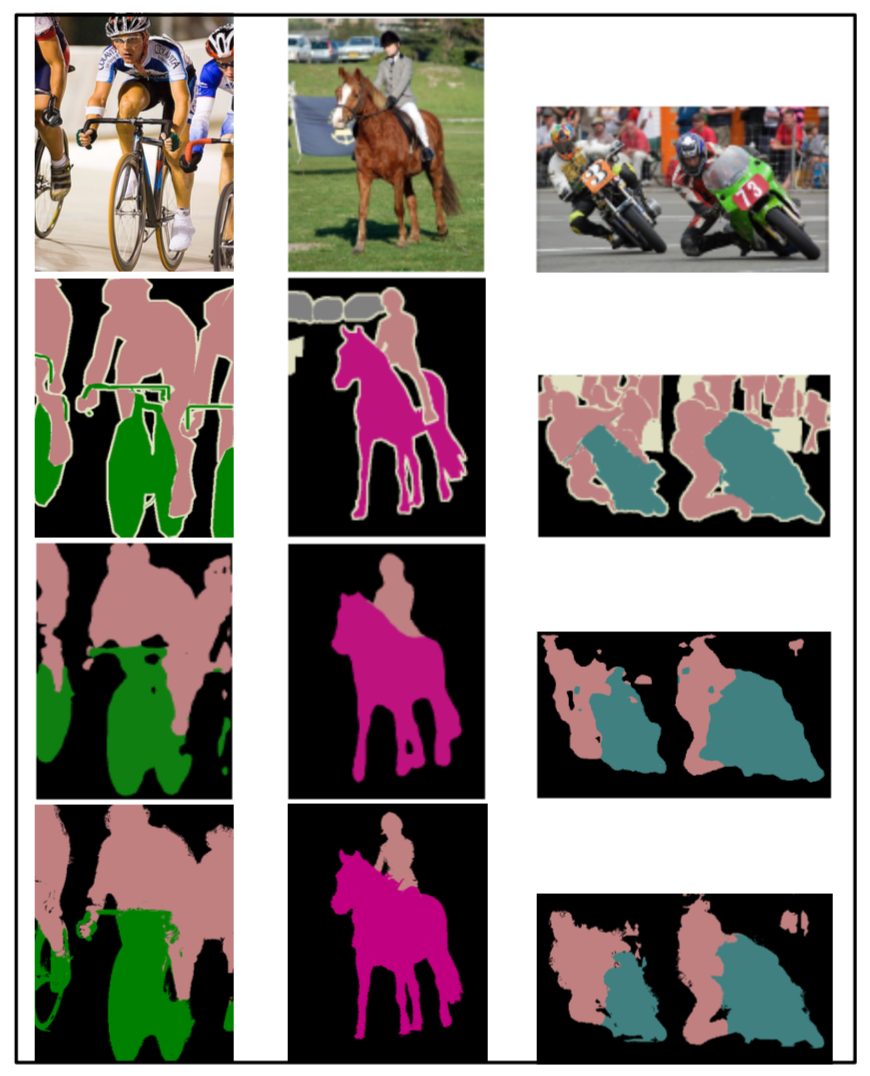
\includegraphics[width=\textwidth]{images/deeplabvsfcn}
	\end{minipage}
	\caption{\label{deeplabvsfcn}DeepLab与FCN在PASCAL VOC数据集上的实验结果对比图。上图为测试指标的对比示意图。下图为实验效果对比图:第一行为原始图像,第二行为ground truth,第三行为FCN分割效果图,第四行为DeepLab分割效果图}
\end{figure}

\section{DilatedConv}
论文Multi-Scale Context Aggregation by Dilated Convolutions\cite{yu2015multi}是收录于ICLR 2016的一篇文章,提出了一种卷积网络模块,可以聚合多尺度的上下文信息,而不会丢失分辨率或重复分析重缩放的图像。该模块基于空洞卷积,其支持指数级扩展感受野而不损失分辨率或覆盖范围。

\subsection{空洞卷积}
与上一节DeepLab中提出的带孔卷积类似,主要目的是增加感受野。传统卷积操作增加感受野的速度是很慢的,所以一般会在卷积层之后增加池化层进一步增加感受野,但是增加池化层之后会使得图像进行了下采样,使得图像丢失了很多细节信息。

设$F:\mathbb{Z}^2\to \mathbb{R}$是一个离散函数,令$\Omega_r=[-r,r]^2\cap \mathbb{Z}^2$,再设$k:\Omega_r\to \mathbb{R}$是一个大小为$(2r+1)^2$的离散滤波器。因此传统的离散卷积操作可以$*$描述为:
\begin{equation}
(F*k)(\mathbf{p})=\sum_{\mathbf{s}+\mathbf{t}=\mathbf{p}}F(\mathbf{s})k(\mathbf{t})
\end{equation}
对其进行拓展,我们可以定义膨胀系数为$l$的空洞卷积运算$*_l$如下:
\begin{equation}
(F*_lk)(\mathbf{p})=\sum_{\mathbf{s}+l\mathbf{t}=\mathbf{p}}F(\mathbf{s})k(\mathbf{t})
\end{equation}

如图\ref{dial}所示展示了膨胀系数为2的空洞卷积操作的示意图,与传统卷积相比,可以看出空洞卷积的卷积核作用于feature map上的物理位置是不连续的。
\begin{figure}[!h]
	\centering
	\begin{minipage}[t]{0.3\textwidth}
		\centering
		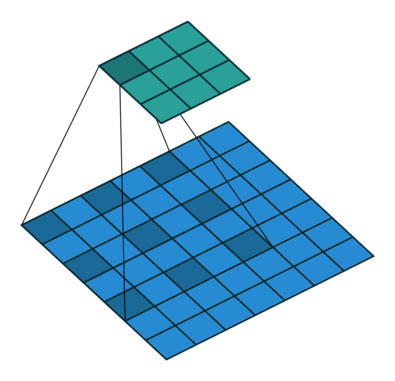
\includegraphics[width=\textwidth]{images/dilation-00.jpg}
	\end{minipage}
	\begin{minipage}[t]{0.3\textwidth}
		\centering
		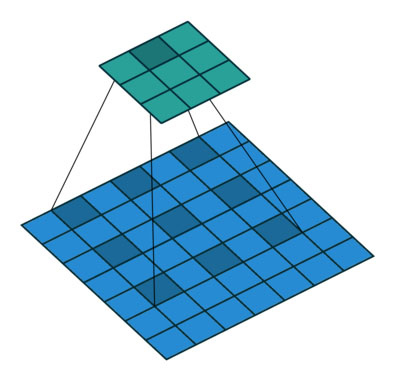
\includegraphics[width=\textwidth]{images/dilation-01.jpg}
	\end{minipage}
	\begin{minipage}[t]{0.3\textwidth}
		\centering
		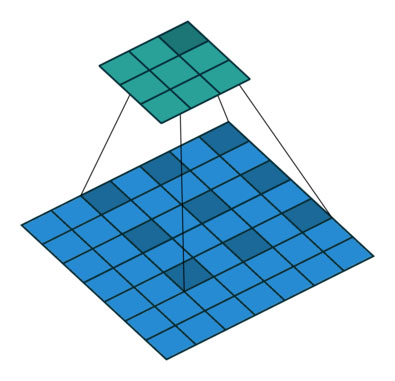
\includegraphics[width=\textwidth]{images/dilation-02.jpg}
	\end{minipage}
	\caption{\label{dial}空洞卷积操作示意图}
\end{figure}

图\ref{dial2}展示了空洞卷积带来感受野变化的示意图。(a)表示普通的卷积,卷积核为$3\times3$,感受野也为 $3\times3$,较小;(b) 表示扩张系数为2 的空洞卷积,卷积核为$3\times3$,但是感受野有$7\times7$,比之前大了一点;(c) 表示扩张系数为 4 的空洞卷积,卷积核为$3\times3$,但是感受野有$15\times15$,更大了。
\begin{figure}[!h]
	\centering
	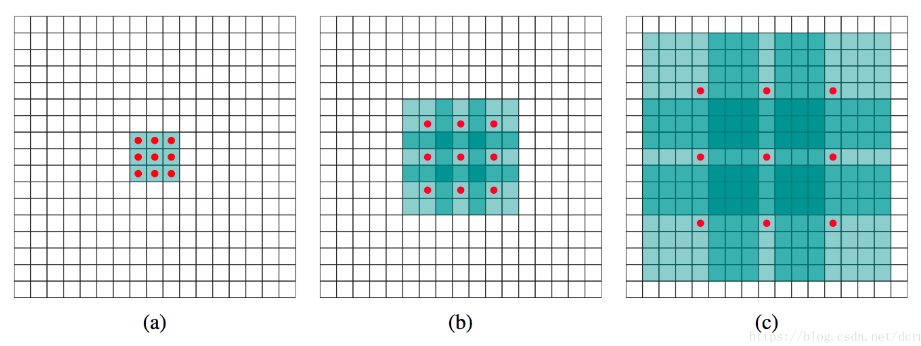
\includegraphics[width=\textwidth]{images/dilateconv}
	\caption{\label{dial2}空洞卷积感受野变化示意图}
\end{figure}
\subsection{网络结构}

DilatedConv的网络结构分为两个模块:front-end模块和Context模块。front-end模块是在VGG\upcite{simonyan2014very}的基础上进行修改得到的,该模块的作用是为了产生feature map为context模块作用。图\ref{deeplabNet}展示了DilatedConv网络结构和原始VGG网络结构的对比。主要进行了如下几点修改:
\begin{itemize}
	\item 与全卷积网络FCN一样,DilatedConv也将VGG中的全连接层修改为卷积层;
	\item 去掉了最后两个池化层;
	\item 将后续的卷积修改为带孔卷积;
	\item 使用ImageNet上预训练的参数进行Finetune。
\end{itemize}

\begin{figure}[!h]
	\centering
	\begin{minipage}[t]{0.45\textwidth}
		\centering
		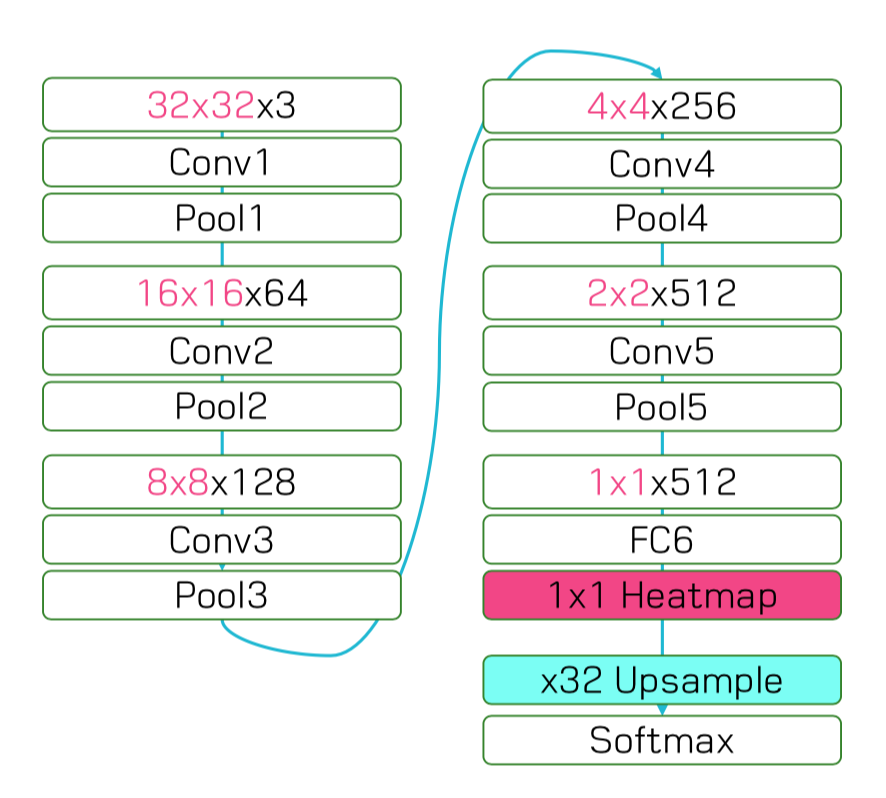
\includegraphics[width=\textwidth]{images/vgg16}
		%		\caption{VGG网络结构图}
	\end{minipage}
	\begin{minipage}[t]{0.45\textwidth}
		\centering
		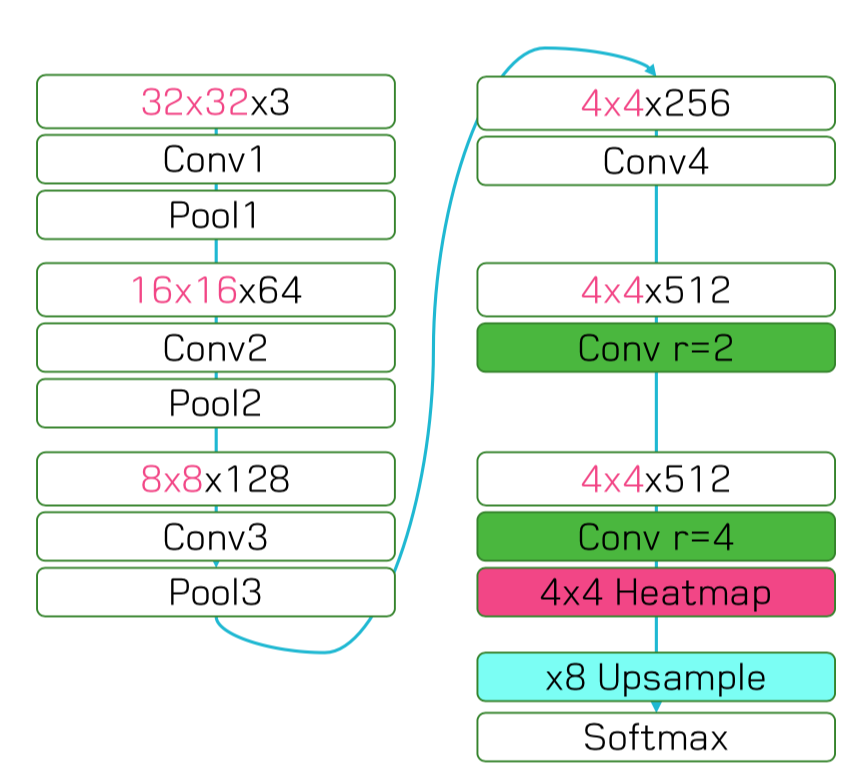
\includegraphics[width=\textwidth]{images/vgg16dial}
		%		\caption{修改之后DeepLab网络结构图}
	\end{minipage}
	\caption{\label{deeplabNet}VGG网络结构示意图和修改之后DilatedConv网络结构实体图的对比图。左图为VGG网络的原始结构示意图,右图为修改之后的DilatedConv网络结构示意图}
\end{figure}

Context模块采用front-end模块输出的feature map作为输入,使用空洞卷积组成8层网络结构,front-end模块和Context模块连接示意图如图\ref{dilate}所示,左图表示front-end模块,可以看出最后输出$64\times64\times C$的feature map,右图表示Context模块,输入为$64\times64\times C$的feature map。
\begin{figure}[!h]
	\centering
	\begin{minipage}[t]{0.45\textwidth}
		\centering
		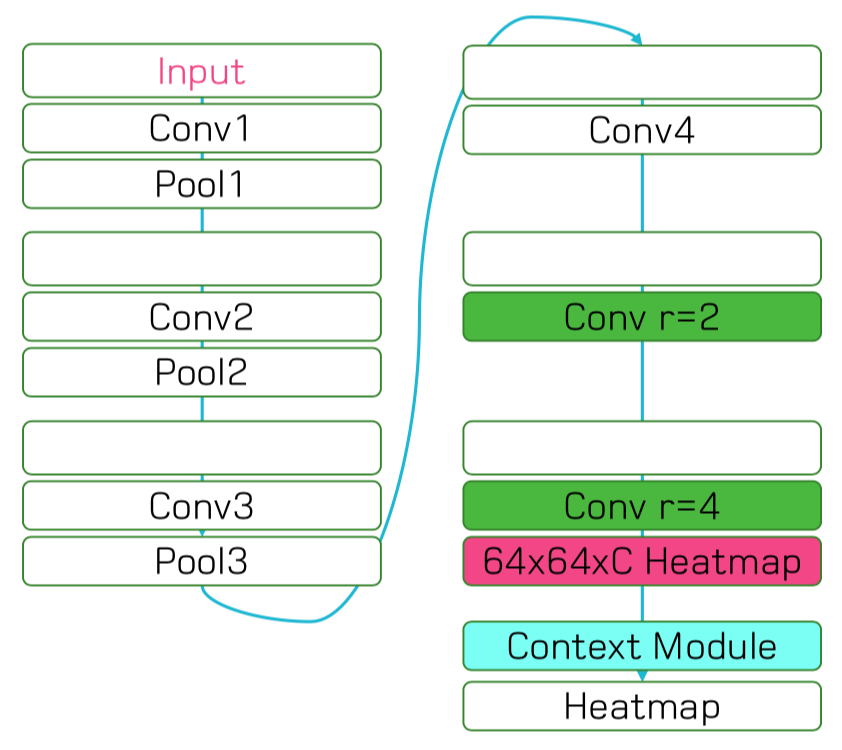
\includegraphics[width=\textwidth]{images/frontmodule}
		%		\caption{VGG网络结构图}
	\end{minipage}
	\begin{minipage}[t]{0.45\textwidth}
		\centering
		\includegraphics[width=\textwidth]{images/Contextmodule}
		%		\caption{修改之后DeepLab网络结构图}
	\end{minipage}
	\caption{\label{dilate}DilatedConv网络front-end模块和Context模块示意图。}
\end{figure}

\subsection{实验结果}
在此,我们将DilatedConv算法的结果与之前提到的FCN和DeepLab进行对比,如图\ref{dilateconv}所示,上图展示了三种算法在PascalVOC数据集上meanIoU的对比情况,可以看出,Dilatedconv算法相比于FCN和DeepLab算法有了进一步的提升,下图表示分割效果的直观对比图,从中我们也能较为清楚的看出,Dilatedconv算法的分割效果有了更进一步的提升。
\begin{figure}[!h]
	\centering
	\begin{minipage}[t]{0.95\textwidth}
		\centering
		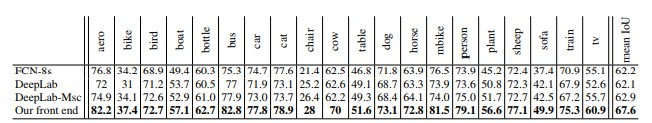
\includegraphics[width=\textwidth]{images/dilatedconv2}
	\end{minipage}
	\begin{minipage}[t]{0.95\textwidth}
		\centering
		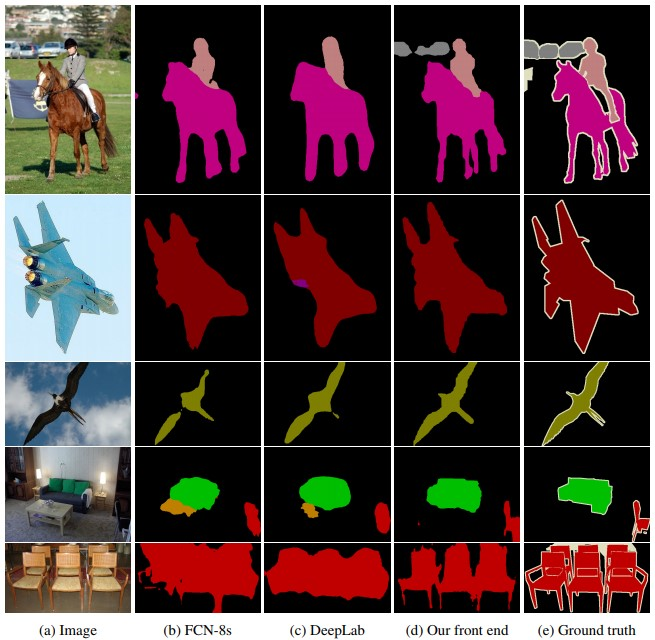
\includegraphics[width=\textwidth]{images/dilatedconv1}
	\end{minipage}
	\caption{\label{dilateconv}DilatedConv算法与FCN、DeepLab算法结果对比图}
\end{figure}

\section{DeepLab v2}
DeepLab v2(DeepLab: Semantic Image Segmentation with Deep Convolutional Nets, Atrous Convolution, and Fully Connected CRFs)\upcite{chen2018deeplab}是DeepLab系列的第二篇文章,最早版本于2016年6月在arXiv上发表,被TPAMI 2017收录。他依然使用了之前提到的全卷积网络、空洞卷积、条件随机场等算法,相比于DeepLab v1,他提出了空洞空间卷积池化金字塔(atrous spatial pyramid pooling (ASPP)),以多尺度的信息得到更强健的分割结果。ASPP并行的采用多个采样率的空洞卷积层来探测,以多个比例捕捉对象以及图像上下文。除此之外,DeepLab v2基础网络结构由VGG16转为ResNet,使用了不同的学习策略,并在使用在MS-COCO数据集上预训练的参数进行finetune。图\ref{deeplabv2}展示了DeepLab v2算法的结构。

\begin{figure}[!h]
	\centering
	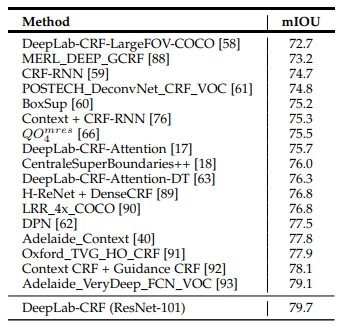
\includegraphics[width=\textwidth]{images/deeplabv2}
	\caption{\label{deeplabv2}DeepLab v2算法结构示意图}
\end{figure}

\subsection{ASPP模块}
受SPPNet中SPP模块的启发,它指出在任意尺度的区域,可以用从单个尺度图像中进行重采样提取的卷积特征进行准确有效地分类。我们用不同采样率的多个并行的空洞卷积实现了他们的方案的一个变体。并行的采用多个采样率的空洞卷积提取特征,再将特征融合,类似于空间金字塔结构。图\ref{aspp1}和图\ref{aspp2}展示了ASPP模块和ASPP模块在网络中结构的示意图。

\begin{figure}[!h]
	\centering
	\begin{minipage}[t]{0.4\textwidth}
		\centering
		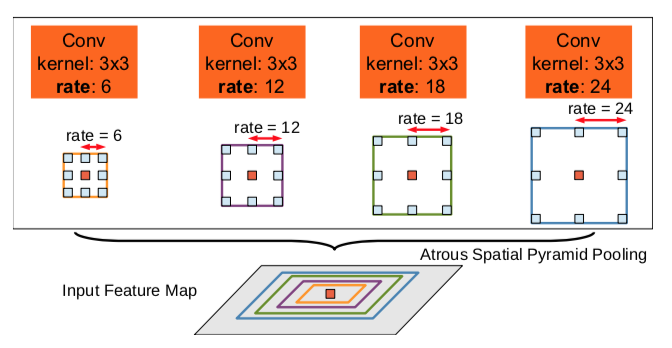
\includegraphics[width=\textwidth]{images/aspp1.png}
		\caption{\label{aspp1}ASPP模块示意图}
	\end{minipage}
	\begin{minipage}[t]{0.4\textwidth}
		\centering
		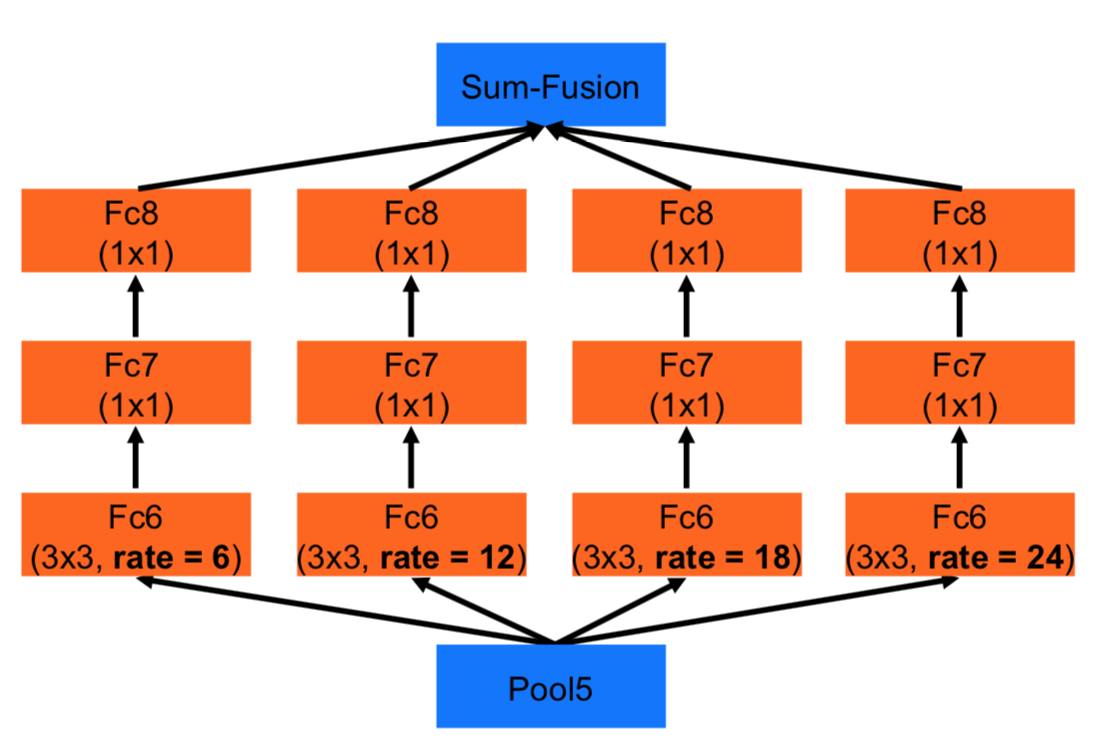
\includegraphics[width=\textwidth]{images/aspp2.png}
		\caption{\label{aspp2}ASPP结构示意图}
	\end{minipage}
\end{figure}

\subsection{实验结果}
DeepLab v2融合了之前算法所提到的模块并且加入了新的ASPP模块,使得分割效果有了进一步的提升。图\ref{deeplabv2res}展示了DeepLab v2算法与之前出现的图像分割算法在PASCAL VOC2012测试集上mIoU的对照表格,从中我们可以看出来,DeepLab v2算法的mIoU值相比于之前的算法都高,因此,其分割效果也得到了进一步的提升。
\begin{figure}[!h]
	\centering
	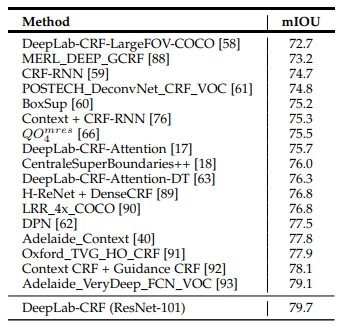
\includegraphics[width=0.8\textwidth]{images/deeplabv2.jpg}
	\caption{\label{deeplabv2res}DeepLab v2算法与之前出现的图像分割算法在PASCAL VOC2012测试集上mIoU的对照表}
\end{figure}

\section{PSPNet}
论文Pyramid Scene Parsing Network\upcite{DBLP:journals/corr/ZhaoSQWJ16}是CVPR2017收录的关于场景解析的文章,拿下了2016年的ImageNet比赛中scene parsing任务的冠军,也可以用于做图像语义分割。这篇文章出发点是在语义分割算法中引入更多的上下文信息(context information), 这样能够避免许多误分割,PSPNet在FCN算法的基础上引入更多上下文信息是通过全局均值池化操作(global average pooling)和特征融合实现的,因此特征呈金字塔结构,这也是论文名叫pyramid的原因。

\subsection{算法结构}
图\ref{pspnet1}展示的PSPNet算法结构示意图。首先输入图像经过一个特征提取网络提取特征,这部分作者采用的是添加了空洞卷积的ResNet网络,提取到的特征(具体而言stride=8)作为后面pyramid pooling模块的输入。在pyramid pooling模块中构建了深度为4的特征金字塔,不同深度的特征是基于输入特征通过不同尺度的池化操作得到的,池化的尺度是可以调整的,这篇文章中给出的池化后的特征尺寸分别是$1\times1$、$2\times2$、$3\times3$和$6\times6$。然后通过一个$1\times1$卷积层将特征维度缩减为原来的1/4,最后将这些金字塔特征直接上采样到与输入特征相同尺寸,然后和输入特征做合并,也就是concat操作得到最终输出的特征图。

\begin{figure}[!h]
	\centering
	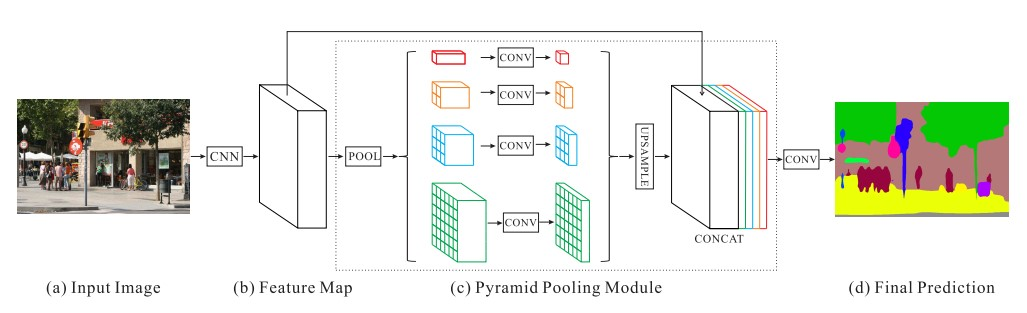
\includegraphics[width=\textwidth]{images/pspnet1.jpg}
	\caption{\label{pspnet1}PSPNet算法结构示意图}
\end{figure}
\subsection{实验结果}
图\ref{pspnet}展示PSPNet和FCN在数据集ADE20k上的实验效果对比,从中可以看出,FCN的分割效果存在着很多的误分割,而PSPNet减少了很多误分割。第一行中FCN算法误将船分割成车,显然一辆车在水上的概率是很小的,这种是属于明显不匹配的误分割。第二行中FCN算法误将摩天大厦分割成建筑物,摩天大厦和建筑物这两个类别本身是比较接近的,这种是属于类别相近的误分割,这部分个人认为是和数据集相关的。第三行中FCN算法误将枕头分割成床,枕头本身区域较小,而且纹理和床较为接近,这种是属于难以觉察的误分割。作者认为这些误分割都可以通过引入更多的上下文信息进行解决,当分割层有更多全局信息时,出现上述几种误分割的概率就会相对低一些,这种思想目前在许多图像领域都有所应用,而引入更多上下文信息的方式也很多,比如:1、增大分隔层的感受野,这种方式是最直观的,视野越广,看到的东西也越多,而增大感受野也有许多方式,比如空洞卷积(dilated convolution),这是在deeplab算法上成功应用的实现方式,另外PSPNet的全局均值池化操作也是增加感受野的一种方式。2、深层特征和浅层特征的融合,增加浅层特征的语义信息,这样在浅层进行分割时就有足够的上下文信息,同时也有目标的细节信息,这种做法早在FCN中就有了,但是包括融合策略和分割层的选择都有一定的优化空间。
\begin{figure}[!h]
	\centering
	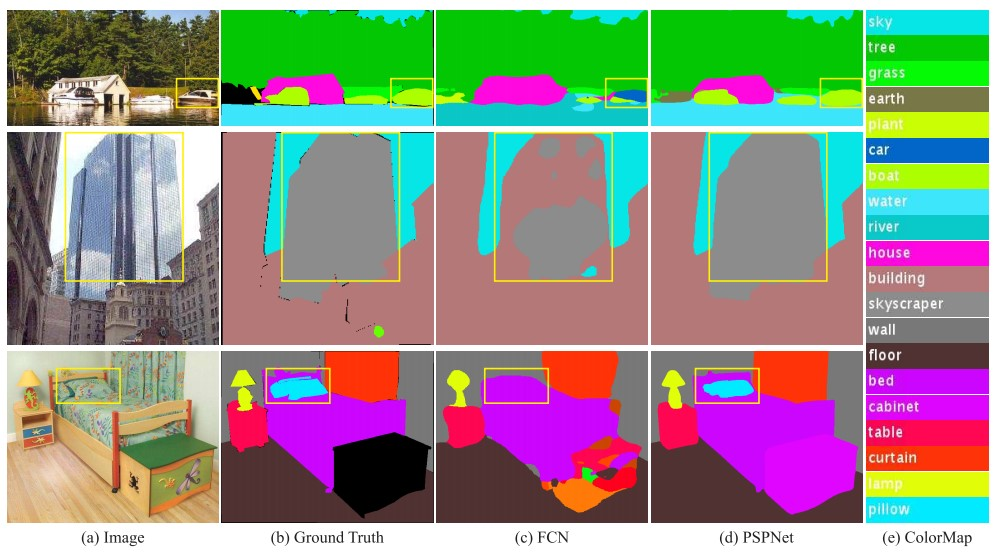
\includegraphics[width=\textwidth]{images/pspnet.jpg}
	\caption{\label{pspnet}PSPNet和FCN在数据集ADE20k上的实验效果对比}
\end{figure}

图\ref{pspnet2}展示了PSPNet和图像分割其他算法在PASCAL VOC 2012测试集上结果比较,表格下半部分表示使用了MS-COCO数据集上预训练的参数进行finetune的结果,可以看出,PSPNet相比于之前出现的算法分割效果的指标有了进一步的提升。
\begin{figure}[!h]
	\centering
	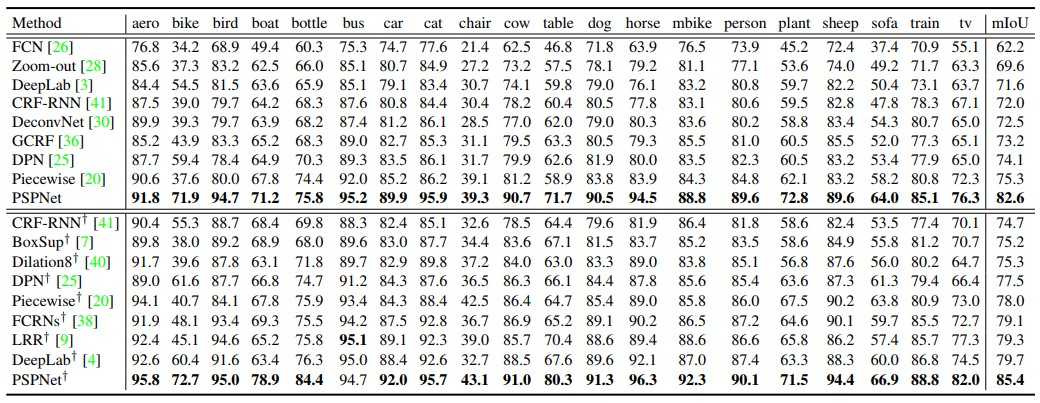
\includegraphics[width=\textwidth]{images/pspnet2.jpg}
	\caption{\label{pspnet2}PSPNet和图像分割其他算法在PASCAL VOC 2012测试集上结果比较}
\end{figure}

\section{DeepLab v3}
DeepLab v3(Rethinking Atrous Convolution for Semantic Image Segmentation)\upcite{chen2017rethinking}是DeepLab系列的第三篇文章,最早在arXiv上发布于2017年6月。相比于之前的算法,主要有以下几点改进:
\begin{itemize}
	\item 提出了更通用的框架,适用于任何网络;
	\item 复制了ResNet最后的block并且级联起来;
	\item 在ASPP模块中使用BN层,并且有了新的ASPP结构;
	\item 取消了后续的DenseCRF,减少了训练时间
\end{itemize}

\subsection{级联模块}
如图\ref{deeplabv3}所示,复制ResNet最后一个block的多个副本,并且级联起来,图\ref{deeplabv3}中的block5-7是block4的副本。每个block中包含三个卷积(MultiGrid),每个block中最后一个卷积的步长为2(最后一个block除外),为了维持原图尺寸,使用不同采样率的空洞卷积来代替原来的卷积。
\begin{figure}[!h]
	\centering
	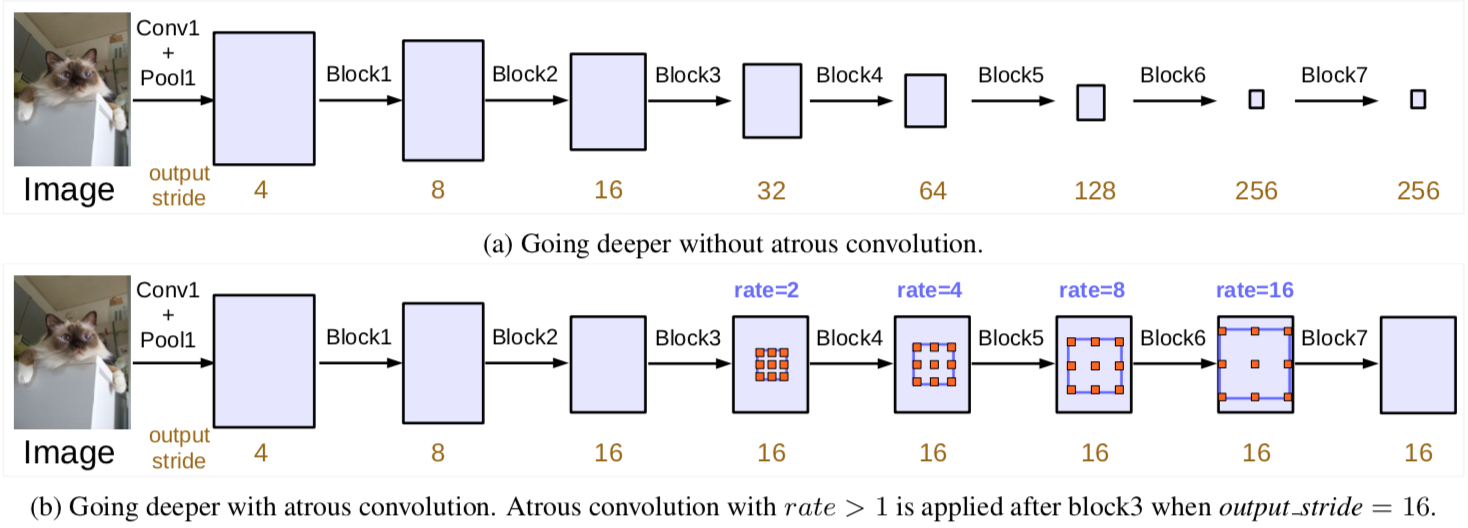
\includegraphics[width=\textwidth]{images/deeplabv3.png}
	\caption{\label{deeplabv3}级联模块使用空洞卷积和不使用空洞卷积的示意图}
\end{figure}

\subsection{新的ASPP模块}
相比于原ASPP模块有如下改变:
\begin{itemize}
	\item ASPP中应用了BN层;
	\item 随着采样率的增加,卷积核中有效的权重减小了;
	\item 使用模型最后的feature map做全局平均池化;
	\item 包括一个$1\times 1$的卷积和3个$3\times 3$采样率分别为(6,12,18)的空洞卷积,并且每个卷积都有BN层和一个全局平均池化层;
	\item 所有的分支通过$1\times 1$的卷积级联起来。
\end{itemize}

\begin{figure}[h]
	\centering
	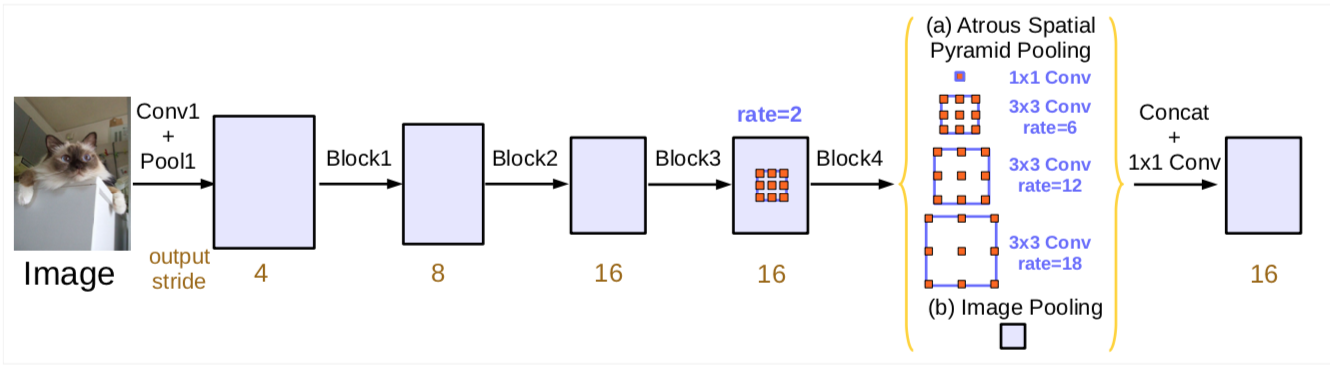
\includegraphics[width=\textwidth]{images/asppnew.png}
	\caption{\label{asppnew}新的ASPP模块}
\end{figure}

\subsection{实验结果}
图\ref{result0}展示了DeepLab v3和之前算法在PASCAL VOC 2012测试集上图像分割性能指标的对比表格,可以看出,DeepLab v3相比于之前的算法,分割的效果有了更进一步的提升,同时,由于其并没有使用CRF,所以训练时间也比DeepLab v1和v2少了很多,因此,DeepLab v3效果的提升是比较大的。图\ref{result1}展示了DeepLab v3在PASCAL VOC数据集上分割效果示意图,可以看出分割的效果相比于最初的FCN已经有了很大的提升,虽然没有使用CRF,但是细节部分分割效果也非常好。
\begin{figure}[h]
	\centering
	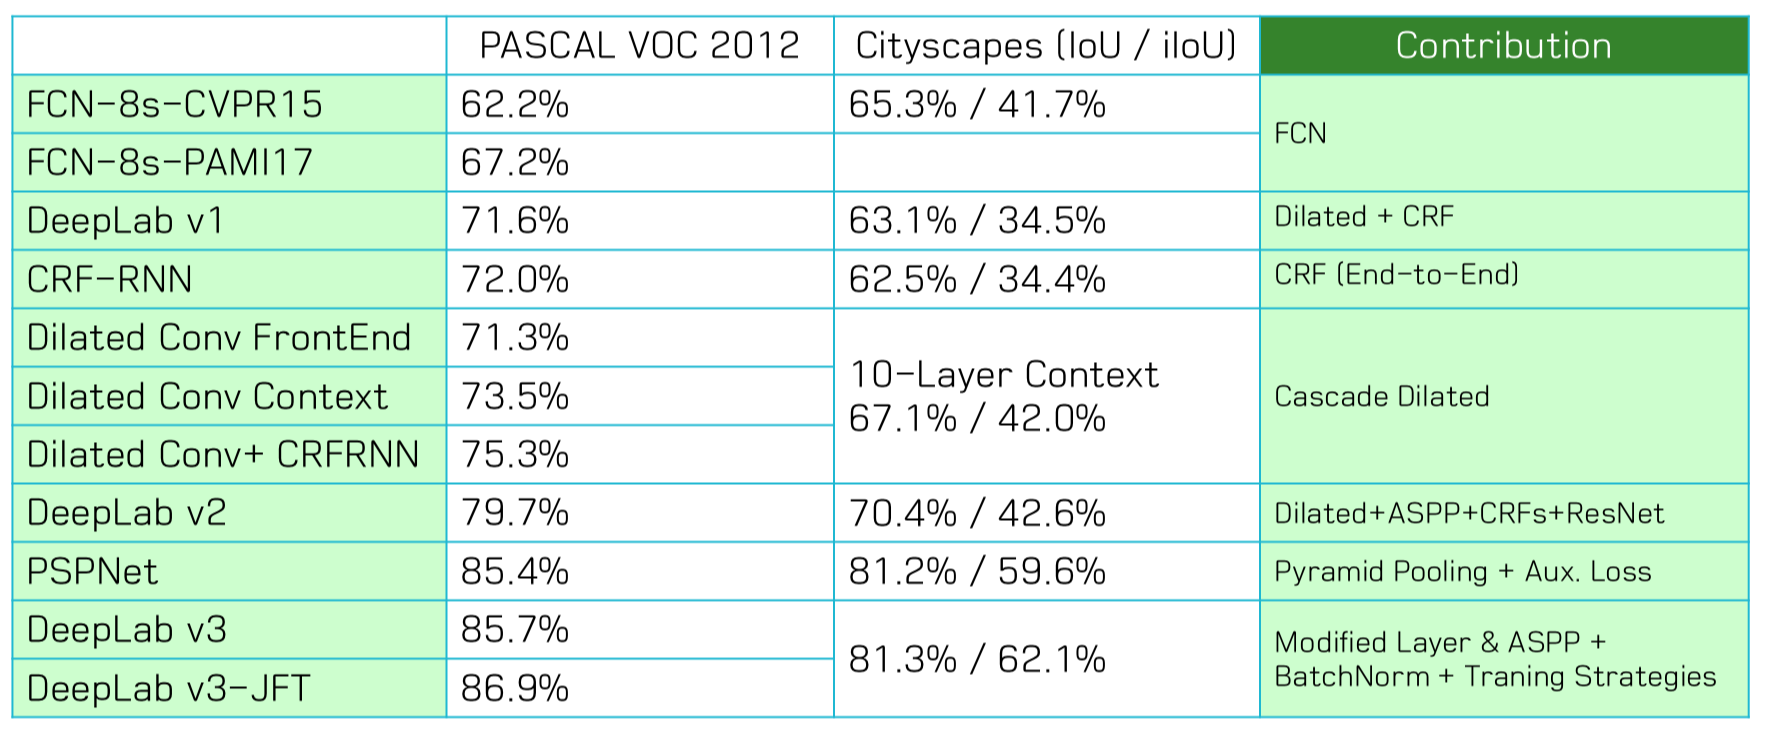
\includegraphics[width=\textwidth]{images/result0.png}
	\caption{\label{result0}PASCAL VOC 2012实验结果对比}
\end{figure}

\begin{figure}[h]
	\centering
	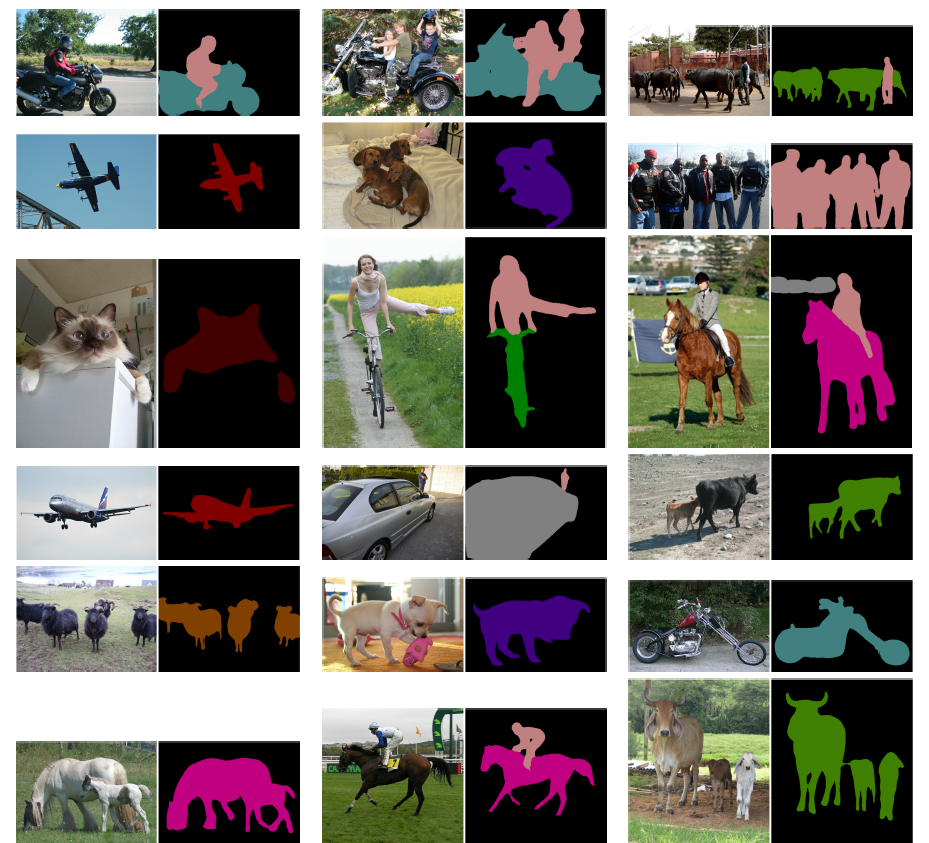
\includegraphics[width=\textwidth]{images/allresults.png}
	\caption{\label{result1}DeepLab v3在PASCAL VOC数据集上分割效果示意图}
\end{figure}

\chapter{最新图像语义分割算法}
上一章主要研究了近几年基于深度学习的图像语义分割算法,并对实验结果进行了对比。在本章主要研究2018年图像分割领域的CVPR、ECCV的文章,调研一下目前图像分割领域的前沿方向。

\section{Depth-aware CNN}
Depth-aware CNN for RGB-D Segmentation\upcite{wang2018depth} 是ECCV 2018上关于图像语义分割的一篇论文,针对RGB-D的图像提出了一种新的算法。

此前关于RGB-D图像的分割方法主要有:
\begin{itemize}
	\item 使用全卷积网络FCN将RGB信息和Depth信息使用两个独立的CNN来进行处理。这样处理会使得参数量和训练时间变为单个CNN的两倍,并且像素之间的关联也因此变弱。
	\item 使用3D networks来处理深度信息,但是这样操作会使得计算复杂度提升很多。
\end{itemize}
这篇论文提出了一种使用2D CNN来处理RGB-D图像语义分割的算法。为了解决像素之间深度信息关联性以及计算复杂度,参数量过多的问题,算法主要采用以下3个方式来解决:
\begin{itemize}
	\item 2D CNN。使用传统的2D卷积神经网络结构不引入新的变量可以解决参数量过多、计算量过大的问题;
	\item depth-aware convolution。定义一种新的卷积方式来处理像素间深度信息关联问题;
	\item depth-aware average pooling。类似于depth-aware convolution,定义一种新的均值池化方式来处理像素间关联的问题。
\end{itemize}

\subsection{Depth-aware Convolution}
图\ref{sconv}所示表示的是正常的卷积操作,按照式(\ref{sconv1})的公式进行计算。其中$\mathcal{R}$是$\mathrm{p}_0$的邻域,$\mathrm{w}$是卷积核。
	\begin{equation}
	\label{sconv1}
	\mathrm{y}(\mathrm{p}_0)=\sum_{\mathrm{p}_n\in \mathcal{R}}\mathrm{w}(\mathrm{p}_n)\cdot \mathrm{x}(\mathrm{p}_0+\mathrm{p}_n)
	\end{equation}
	图\ref{dconv}所示表示的是Depth-aware的卷积操作,按照式(\ref{dconv:eq})的公式进行计算。
	\begin{equation}
	\label{dconv:eq}
	\mathrm{y}(\mathrm{p}_0)=\sum_{\mathrm{p}_n\in \mathcal{R}}\mathrm{w}(\mathrm{p}_n)\cdot \mathrm{F_D}(\mathrm{p}_0,\mathrm{p}_0+\mathrm{p}_n)\cdot\mathrm{x}(\mathrm{p}_0+\mathrm{p}_n)
	\end{equation}
	其中$\mathrm{F_D}$表示像素之间深度信息的关联,如式(\ref{depthFunction})所示。
	\begin{equation}
	\label{depthFunction}
	\mathrm{F_D}(\mathrm{p}_i,\mathrm{p}_j)=\exp(-\alpha|\mathrm{D}(\mathrm{p}_i)-\mathrm{D}(\mathrm{p}_j)|)
	\end{equation}
	
\begin{figure}[h]
	\centering
	\begin{minipage}[t]{0.4\textwidth}
		\centering
		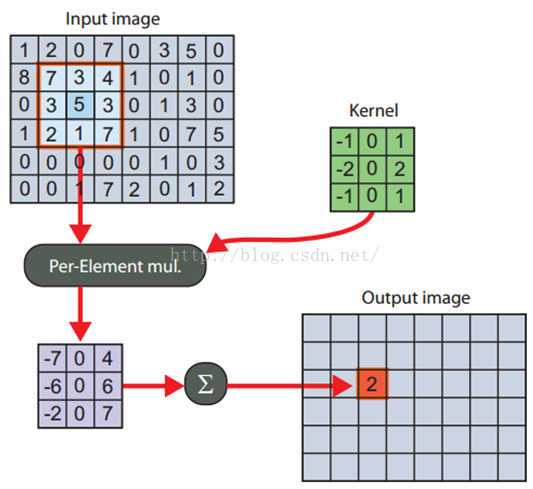
\includegraphics[width=\textwidth]{images/sconv.png}
		\caption{\label{sconv}传统的卷积操作}
	\end{minipage}
	\begin{minipage}[t]{0.4\textwidth}
		\centering
		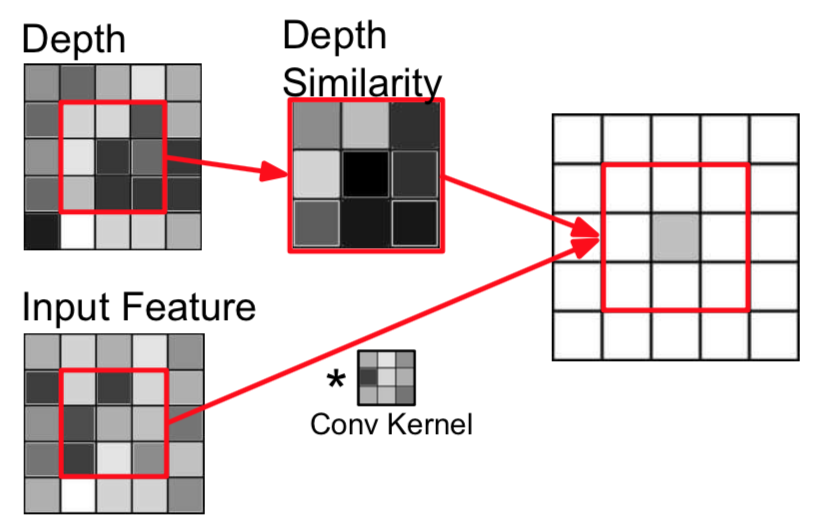
\includegraphics[width=\textwidth]{images/dconv.png}
		\caption{\label{dconv}depth-aware卷积操作}
	\end{minipage}
\end{figure}
\subsection{Depth-aware Average Pooling}
与Depth-aware卷积类似,Depth-aware平均值池化也引入了深度信息。图\ref{savg}所示表示的是正常的平均值池化操作,按照式(\ref{savg1})的公式进行计算。其中 $\mathcal{R}$是$\mathrm{p}_0$的邻域。
\begin{equation}
\label{savg1}
\mathrm{y}(\mathrm{p}_0)=\frac{1}{|\mathcal{R}|}\sum_{\mathrm{p}_n\in \mathcal{R}} \mathrm{x}(\mathrm{p}_0+\mathrm{p}_n)
\end{equation}
图\ref{davg}所示表示的是Depth-aware的平均值池化操作,按照式(\ref{davg:eq})的公式进行计算,其中$\mathrm{F_D}$也表示式(\ref{depthFunction})所示的像素之间深度信息的关联。
\begin{equation}
\label{davg:eq}
\mathrm{y}(\mathrm{p}_0)=\frac{1}{|\mathcal{R}|}\sum_{\mathrm{p}_n\in \mathcal{R}} \mathrm{F_D}(\mathrm{p}_0,\mathrm{p}_0+\mathrm{p}_n)\cdot\mathrm{x}(\mathrm{p}_0+\mathrm{p}_n)
\end{equation}
\begin{figure}[h]
	\centering
	\begin{minipage}[t]{0.4\textwidth}
		\centering
		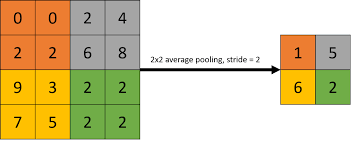
\includegraphics[width=\textwidth]{images/savg.png}
		\caption{\label{savg}传统的均值池化操作}
	\end{minipage}
	\begin{minipage}[t]{0.4\textwidth}
		\centering
		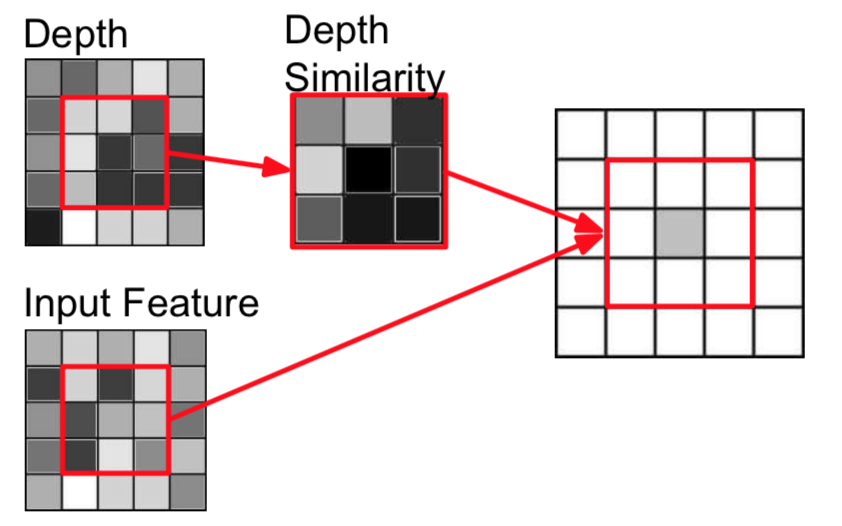
\includegraphics[width=\textwidth]{images/davg.png}
		\caption{\label{davg}depth-aware均值池化操作}
	\end{minipage}
\end{figure}
\subsection{网络结构}
本算法使用DeepLab作为baseline,使用了VGG16和ResNet-15的网络结构,将其中的卷积操作改为式\ref{dconv:eq}中的卷积操作,将其中的均值池化操作改为式(\ref{davg:eq})中的均值池化操作。网络结构如图\ref{arch}所示。

\begin{figure}[h]
	\centering
	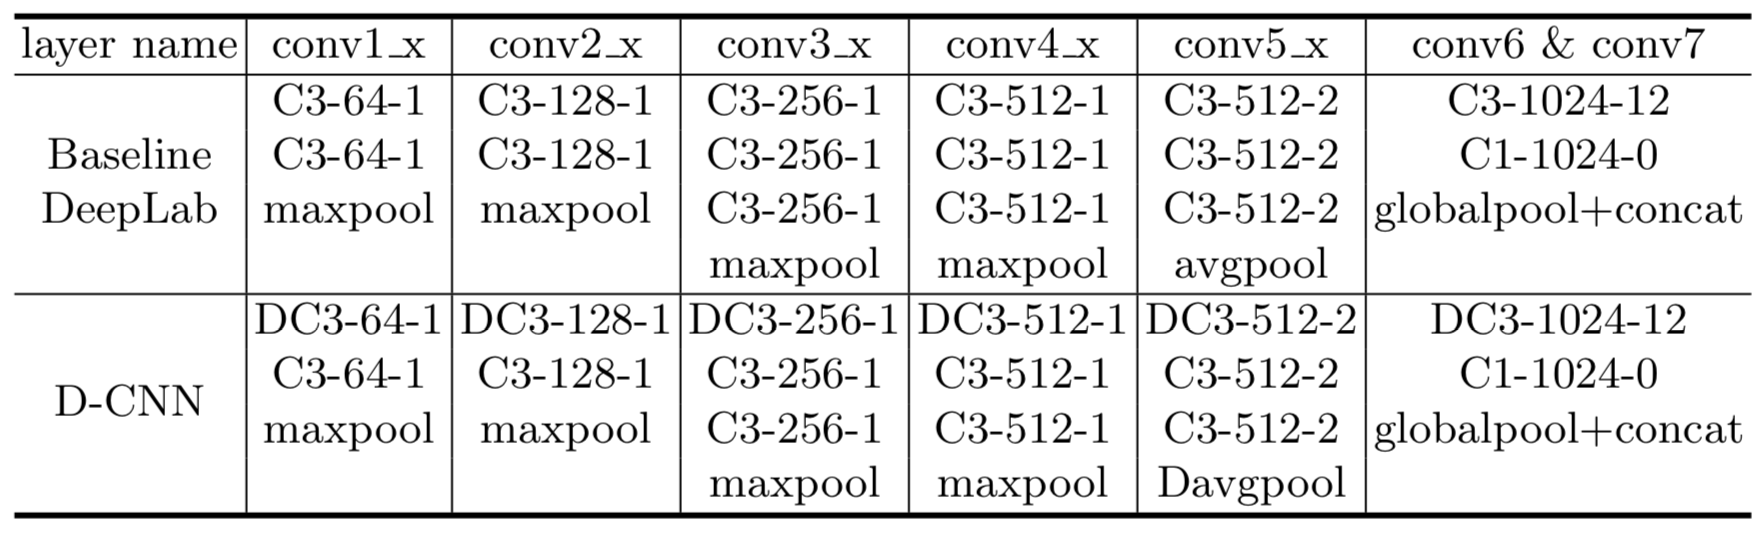
\includegraphics[width=0.9\textwidth]{images/arch.png}
	\caption{\label{arch}DeepLab和DCNN使用VGG16的结构}
\end{figure}

\subsection{实验结果}
本篇论文将提出的算法与DeepLab的baseline在NYUv2\upcite{silberman2012indoor}数据集上进行测试,NYUv2数据集包括1449像素集标注的RGB-D图像,实验按照40个class,将数据划分为训练集:795张图像和测试集:654张图像进行实验得到如图\ref{res1}和图\ref{res2}所示的结果。从图\ref{res1}中可以看出,修改了卷积操作和均值池化操作之后,在具有深度信息的图片上分割指标相比于上一章的DeepLab网络有了很大的提升。

\begin{figure}[h]
	\centering
	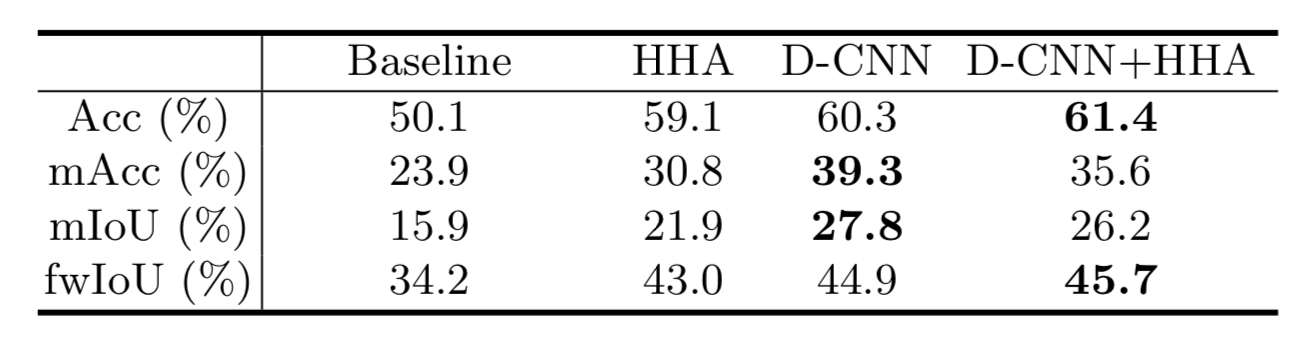
\includegraphics[width=\textwidth]{images/res1.png}
	\caption{\label{res1}DeepLab和DCNN在评价指标上的对比结果}
\end{figure}

从图\ref{res2}中可以直观的看出,加入了深度信息的Depth-aware卷积和Depth-aware均值池化使得图像分割效果有了很大的提升。从中我们也能看出,当我们能够获得的先验信息更多的时候,选择能够利用较多信息的算法可以为我们的识别算法带来很大的提升。
\begin{figure}[h]
	\centering
	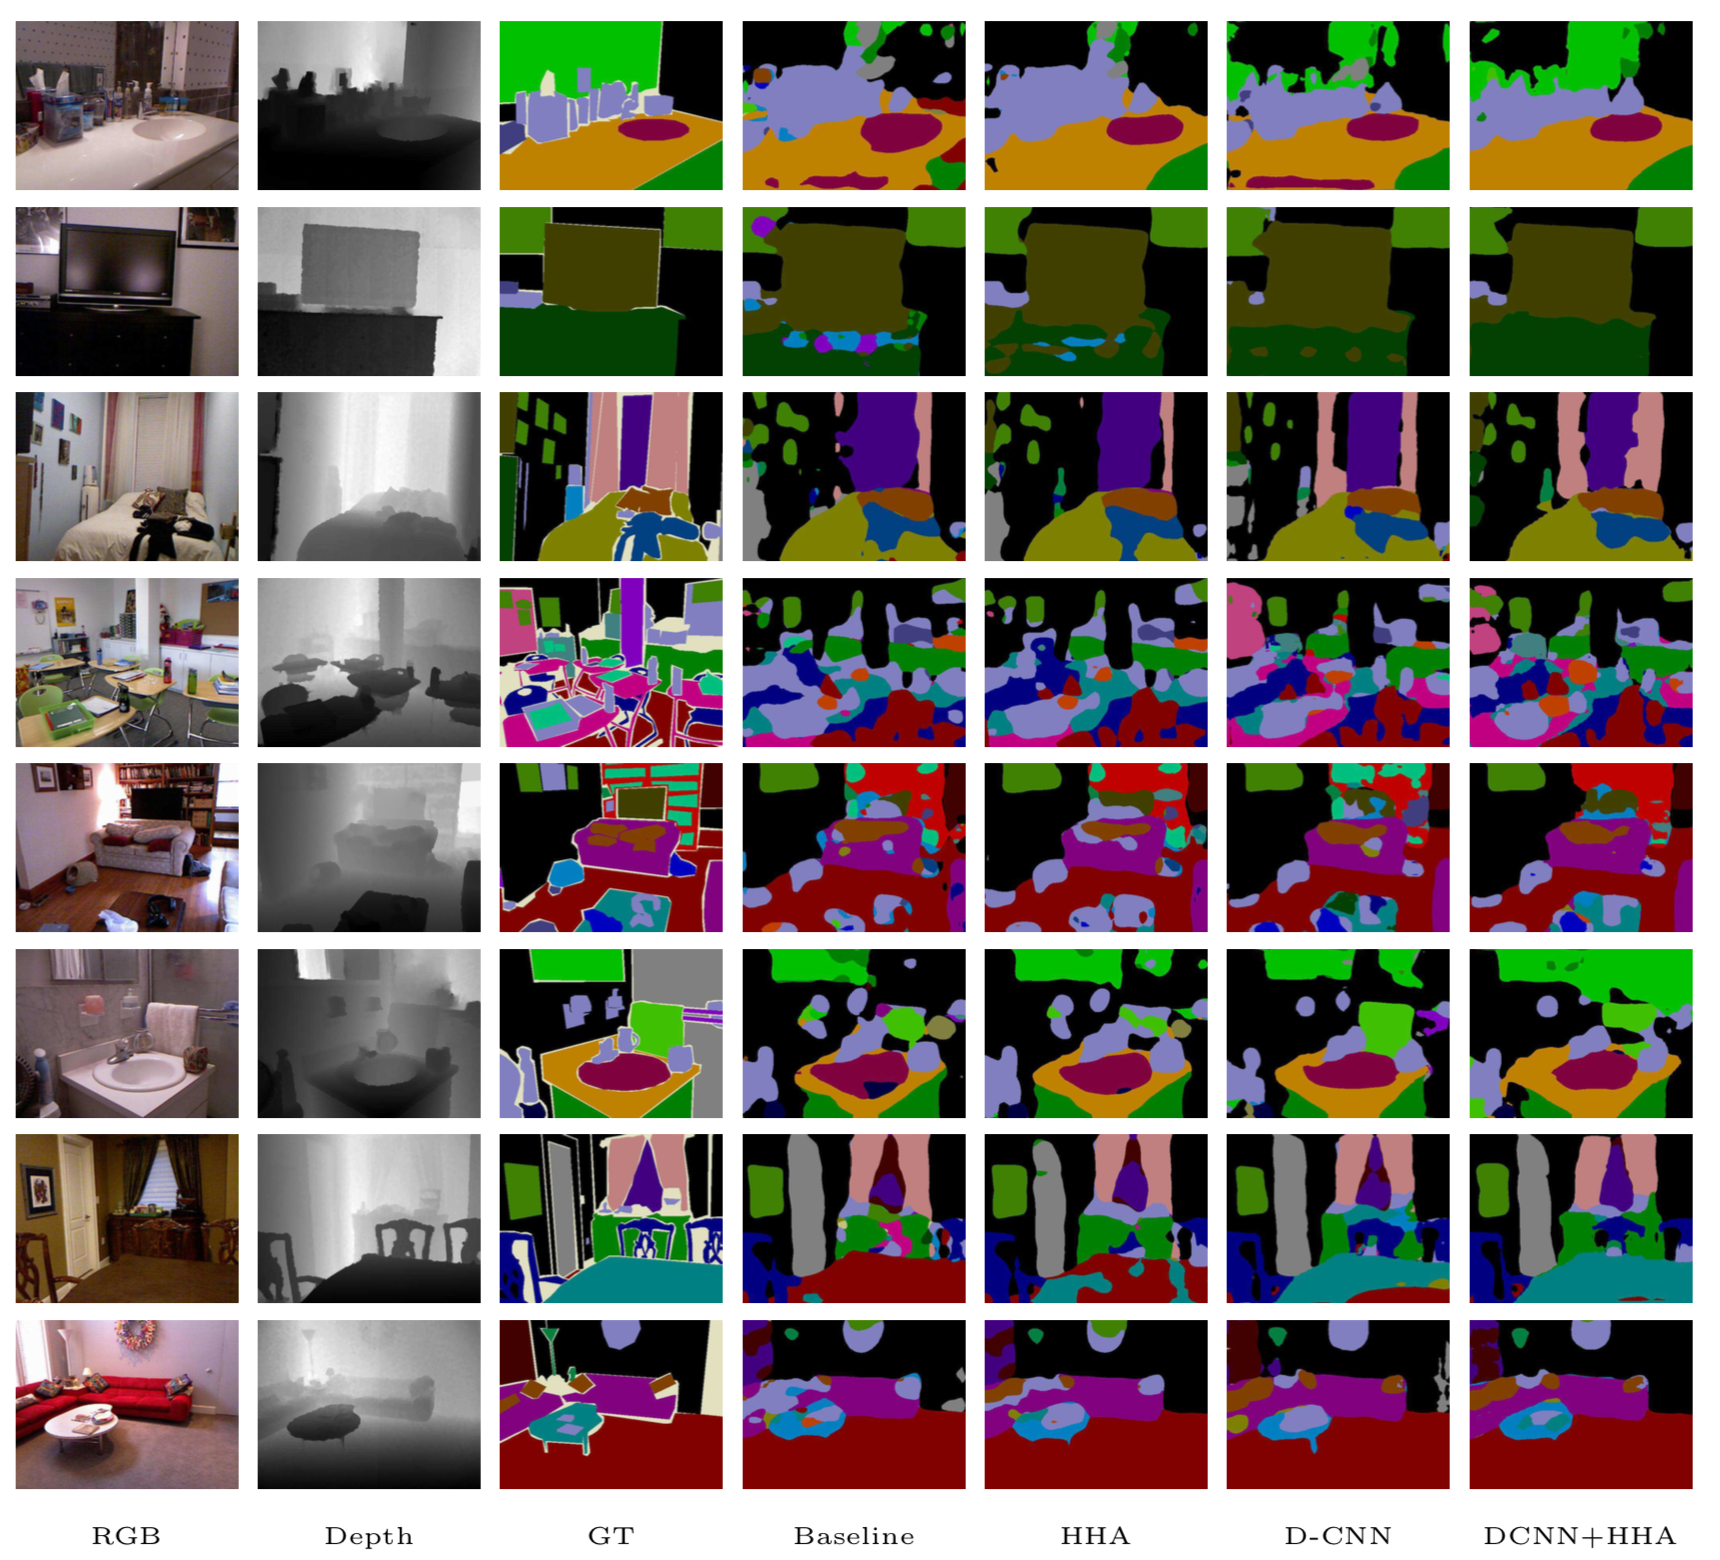
\includegraphics[width=\textwidth]{images/res2.png}
	\caption{\label{res2}DeepLab和DCNN在测试集上的效果图}
\end{figure}

\section{AUNet}
Attention-guided Unified Network for Panoptic Segmentation\cite{li2018attention} 是CVPR2019上的文章。中国科学院自动化研究所所做关于全景分割问题。本文提出了一个叫做 Attention-guided Unified Network (AUNet) 的结构去解决全景分割问题,该方法在MS-COCO数据集上取得了目前最好的结果。

本篇文章涉及到一种新的图像分割方式——图像全景分割(Panoptic Segmentation)。全景分割是一个比较新的分割概念,是指的对目标区域做实例分割(Instance Segmentation),对背景区域做语义分割(Semantic Segmentation)。如图\ref{paseg}所示,图(a)表示输入图片;图(b)表示全景分割的图片,可以看出,很多人在沙滩上放风筝,其中人和风筝是前景,而天空沙滩和远处的森林是背景,在背景的分割中,我们需要区分哪里是沙滩、天空和森林就行了,不需要具体指出有几棵树分别在哪里也就是所谓的语义分割。在前景的分各种,我们不仅仅要指出哪些是人,同时还要把不同的人区分标记,即要数出一共有几个人(这里人就是所谓的实例)也就是实例分割;图(c)表示对前景照片进行实例分割的结果;图(d)表示对背景图进行语义分割的结果。

\begin{figure}[h]
	\centering
	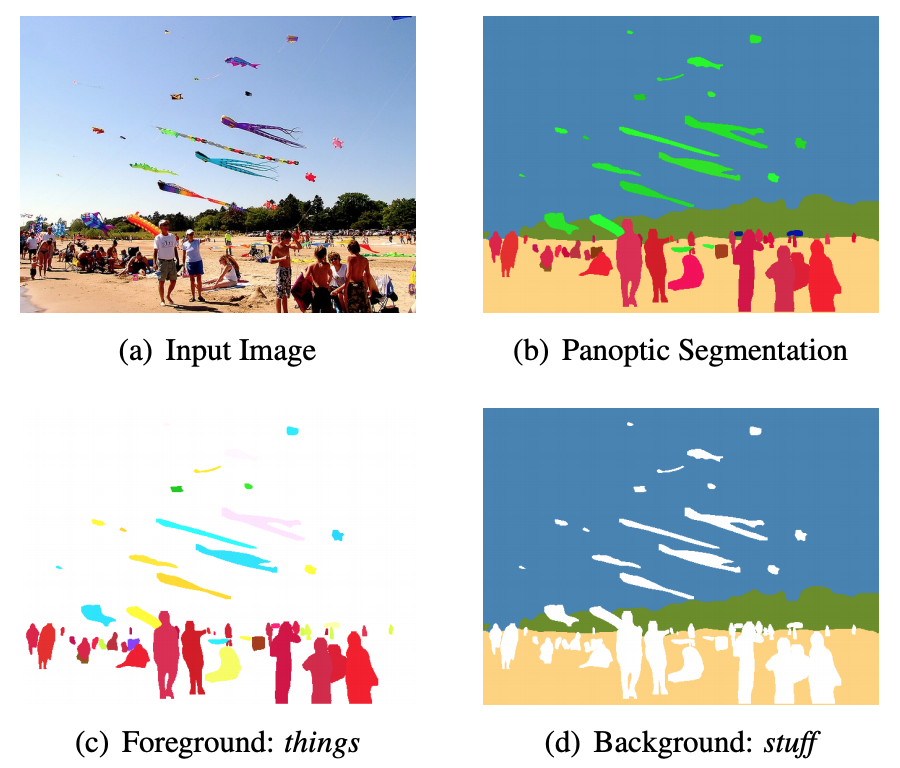
\includegraphics[width=0.8\textwidth]{images/paseg}
	\caption{\label{paseg}图像全景分割示意图}
\end{figure}

之前的对于全景分割的很多工作只是把实例分割和语义分割加在一起,但是并没有考虑二者内在的上下文信息的关系,比如说虽然树木和草地都是绿油油的有点相似,但是人只会站在草地上而不会站在树上。作者也是基于此提出了把语义分割和实例分割二者融合在一起的模型。同时,这篇文章也探讨了如何通过注意力机制实现用高层的图像特征提高分割的准确性。

\subsection{网络结构}

\begin{figure}[h]
	\centering
	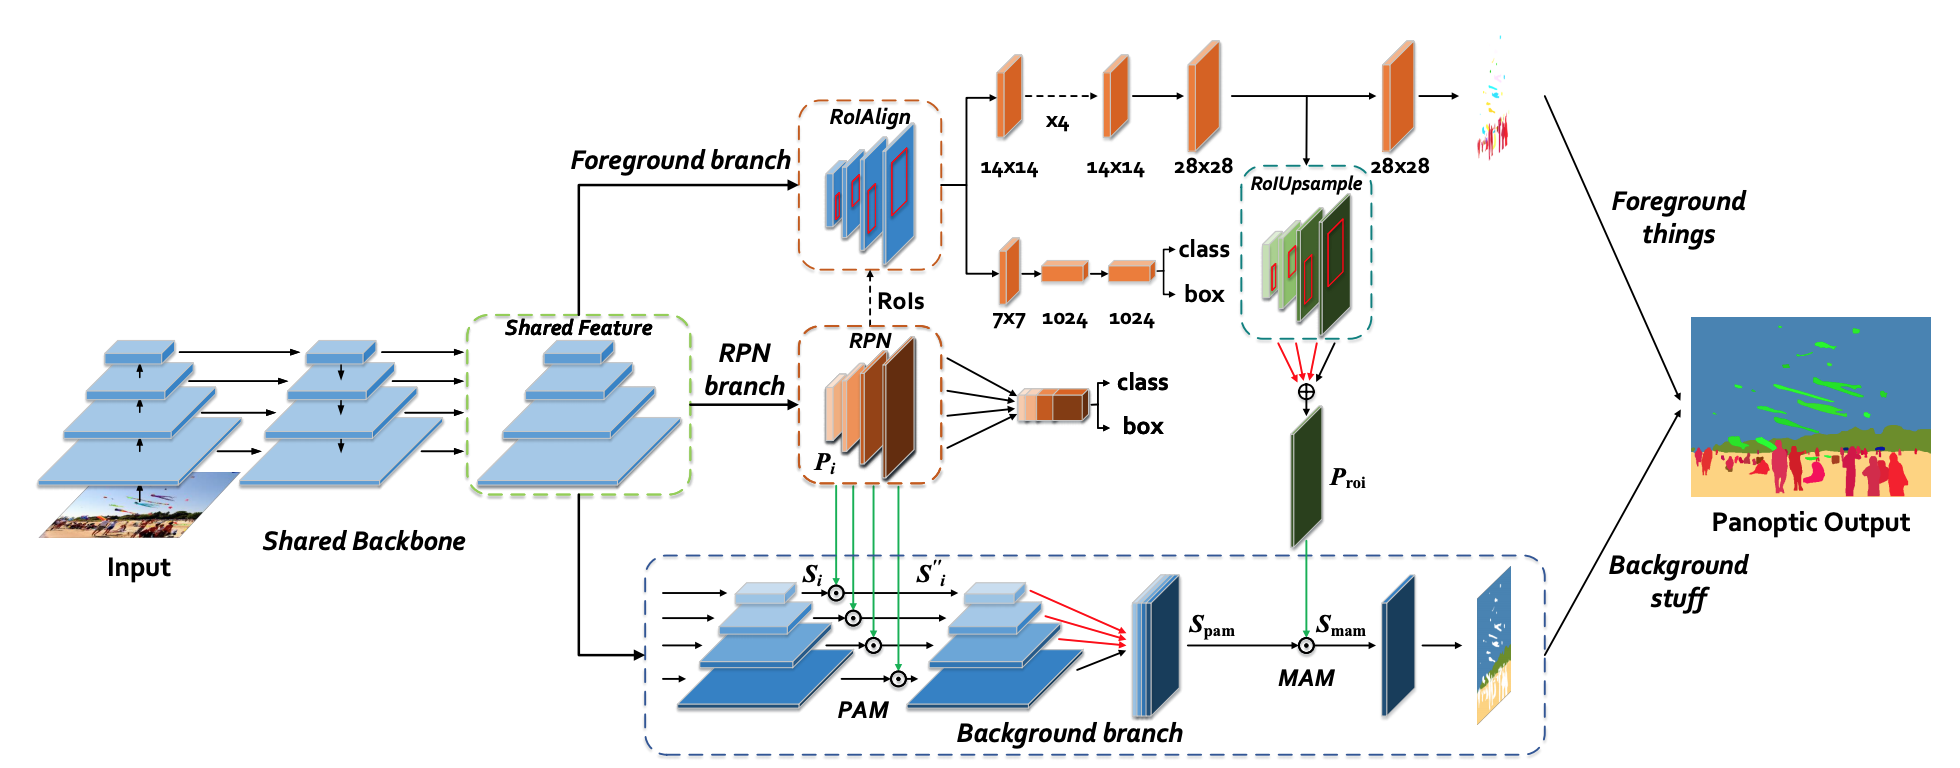
\includegraphics[width=\textwidth]{images/aunet}
	\caption{\label{aunet}AUNet网络结构示意图}
\end{figure}

AUNet的网络结构如图\ref{aunet}所示。该方法以特征金字塔(FPN)作为主干,之后分为了三个分支,分别叫做前景的分支,背景分支和RPN(faster-RCNN中的结构)分支。其中如前文提到的,作者用了两个注意力机制,试图互补前景的信息和背景的信息,其中一个方法叫做PAM(Proposal Attention Module)一个叫做MAM(Mask Attention Module)。

\subsection{Proposal Attention Module}
PAM注意力机制的方法如图\ref{pam}所示,这个注意力模块连接了RPN分支和背景分支。和大部分的注意力机制一样,作者将RPN分支的信息通过制作一个蒙版Mi作用于背景分支(注意这里的蒙版用的是$1-sigmoid$因为RPN选择的前景信息,作为背景蒙版的时候应该用1减去)。这样使得分割任务集中更多注意力在局部目标上,以促进背景语义分割的准确性。在PAM的后面还加入了一个小的结构叫做背景选择,旨在过滤掉没有用的背景特征。
\begin{figure}[h]
	\centering
	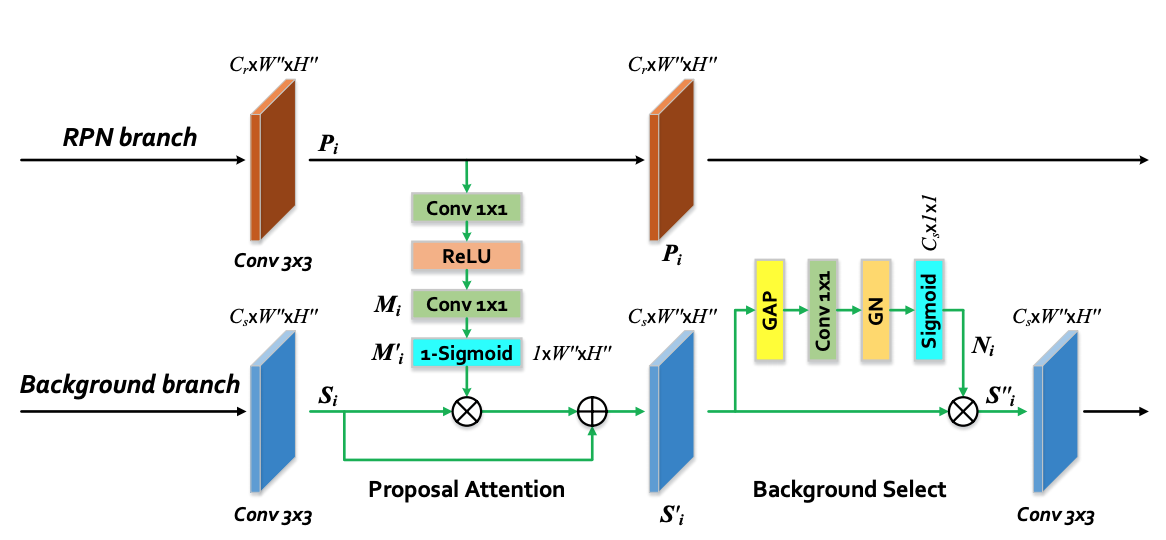
\includegraphics[width=\textwidth]{images/pam}
	\caption{\label{pam}PAM结构示意图}
\end{figure}

\subsection{Mask Attention Module}
MAM注意力模块连接了前景和背景分支,旨在互补二者的信息,方法与之前的类似,同时也用的$1-sigmoid$,还有背景选择,如图\ref{mam}所示。

\begin{figure}[h]
	\centering
	\includegraphics[width=\textwidth]{images/mam}
	\caption{\label{mam}MAM结构示意图}
\end{figure}

同时在MAM中,为了解决在目标检测任务中的ROI尺寸的问题,作者又提出了另外一种插值的方法,叫做RoIUpsample, 用于解决尺寸不同的问题。如图\ref{roiupsample}(b)所示表示的是提出的RoIUpsample算法的示意图,可以将其看做是RoIAlign的逆运算(图\ref{roiupsample}(a)图所示的为RoIAlign操作)。

\begin{figure}[!ht]
	\centering
	\includegraphics[width=0.8\textwidth]{images/roiupsample}
	\caption{\label{roiupsample}RoIUpsample算法示意图}
\end{figure}

\subsection{实验结果}
本篇文章中提出了一个针对图像全景分割的新的评价指标——全景率(panoptic quality),可以同时评价目标检测的好坏和分割结果的好坏,是一个比较综合的指标。计算方式如式(\ref{eq3_2})所示
\begin{equation}
\label{eq3_2}
PQ=\underbrace{\frac{\sum_{(p,q)\in TP}IoU(p,q)}{|TP|}}_{\mbox{segmentation quality(SQ)}}\times\underbrace{\frac{|TP|}{|TP|+\frac{1}{2}|FP|+\frac{1}{2}|FN|}}_{\mbox{recognition quality(RQ)}}
\end{equation}
并且,本篇文章中提到的各个模块没有使用单独的loss,而是使用了统一的loss,这也更加说明这是一个统一的模型,是一个端到端的网络。文章中定义的loss计算如式(\ref{eq3_3})所示。
\begin{equation}
\label{eq3_3}
\mathcal{L}=\lambda_1\mathcal{L}_{cls}+\lambda_2\mathcal{L}_{box}+\lambda_3\mathcal{L}_{mask}+\lambda_4\mathcal{L}_{seg}
\end{equation}
其中$\mathcal{L}_{cls},\mathcal{L}_{box},\mathcal{L}_{mask},\mathcal{L}_{seg}$分别代表object classification, bonding-box regression, instance segmentation, 和semantic segmentation阶段的loss。

本篇文章的实验结果如图\ref{aunetres1},\ref{aunetres2},\ref{aunetres3}所示。图\ref{aunetres1}表示的是仅使用PAM注意力机制得到的实验结果图,从图中可以看出分割的效果还是很好的,使用PAM之后对图像语义分割和实例分割的效果都有一定程度的提升。图\ref{aunetres2}表示的是仅使用MAM注意力机制得到的实验结果图,从图中可以看出,使用MAM之后对前景和背景的层次感有了更好的分割效果。图\ref{aunetres3}展示了本文提出的算法在MS-COCO验证集上的分割效果,可以看出,分割效果相比于我们上一章讨论到的算法有了很大的提升。
\begin{figure}[!h]
	\centering
	\includegraphics[width=\textwidth]{images/aunetres1}
	\caption{\label{aunetres1}使用PAM的实验结果示意图}
\end{figure}
\begin{figure}[!h]
	\centering
	\includegraphics[width=\textwidth]{images/aunetres2}
	\caption{\label{aunetres2}使用MAM的实验结果示意图}
\end{figure}
\begin{figure}[!h]
	\centering
	\includegraphics[width=\textwidth]{images/aunetres3}
	\caption{\label{aunetres3}AUNet在MS-COCO验证集上的结果示意图}
\end{figure}

\section{DANet}
论文Dual Attention Network for Scene Segmentation\cite{fu2018dual}是CVPR 2019上的文章。本篇文章提出了一种使用注意力机制来提高图像语义分割效果的算法,达到了state-of-the-art的水平,主要有两个创新的模块:
\begin{itemize}
	\item \textbf{Position attention module}:捕获特征图的任意两个位置之间的空间依赖,对于某个特定的特征,被所有位置上的特征加权和更新。权重为相应的两个位置之间的特征相似性。因此,任何两个现有相似特征的位置可以相互贡献提升,而不管它们之间的距离。
	\item \textbf{Channel attention module}:捕获任意两个通道之间的相互依赖,利用所有通道的加权和更新某个通道的值。
\end{itemize}

\subsection{网络结构}
如图\ref{danet}所示的为DANet设计的网络结构示意图,左侧ResNet部分使用了上一章提到的带有空洞卷积的全卷积网络,在ResNet之后引入两个注意力机制的模块,最后将两个模块的结果进行sum,得到最终的结果。
\begin{figure}[!h]
	\centering
	\includegraphics[width=\textwidth]{images/danet}
	\caption{\label{danet}DANet网络结构示意图}
\end{figure}

\subsection{Position attention module(PAM)}
如图\ref{pam2}所示是DANet中Position Attention模块的示意图,上下文关系对于场景理解是重要的,旨在捕获全局依赖而无论距离位置。为了建模更丰富的局部上下文依赖,提出PAM模块,编码更宽的上下文依赖到局部特征。
\begin{figure}[!h]
	\centering
	\includegraphics[width=\textwidth]{images/pam2}
	\caption{\label{pam2}DANet Position attention module 示意图}
\end{figure}
具体地,对于网络输出的局部特征$A(C\times H\times W)$,首先利用三个卷积层后得到$B,C,D$三个feature map。然后,对$B,C,D$分别reshape到$(C\times N)$,然后将$B$的转置与$C$相乘后,再通过softmax得到spatial attention map $S(N,N)$,接着,将$S$的转置与$D$矩阵乘后,将结果reshape到$(C\times H\times W)$,乘以一个尺度因子后再加上原始输入图像得到最后的输出map $E$。其中,$S$矩阵的各个元素计算如式(\ref{eq_s})所示,$s_{ji}$表示位置$i$对位置$j$的影响。求出的$S$矩阵相当于一个attention,它的每一行计算的是,所有像素与某个像素之间的依赖关系,使用softmax的作用是类似于分类,softmax值越大,说明更可信。而相对的依赖性也更强。因此,S矩阵的所有行表示了像素与其他像素的依赖关系。注意:在计算$S$时,某个像素特征值使用的是通道维度的值,不是单一的某个通道。最后将attention与原始map相乘,即将所有位置的加权和更新原像素特征值,相当于利用学习到的长距离依赖关系,作用于原始map,选择性的加强局部特征的全局依赖关系。
\begin{equation}
\label{eq_s}
s_{ji}=\frac{\exp(B_i\times C_i)}{\sum_{i=1}^N\exp(B_i\times C_i)}
\end{equation}
\subsection{Channel attention module(CAM)}
如图\ref{cam}所示表示的是DANet中Channel attention module的示意图。高层特征的每个通道可以被视为一个特定类别的响应,不同语义响应相互联系。通过利用不同通道间的依赖关系,可以增强相互依赖的特征通道并且改进特征语义的特征表达。
\begin{figure}[!h]
	\centering
	\includegraphics[width=\textwidth]{images/cam}
	\caption{\label{cam}DANet Channel attention module 示意图}
\end{figure}
先对$A$进行reshape到$(C\times N)$,然后$A$与$A^T$进行矩阵乘,经过softmax后得到通道间的map $X(C\times C)$,之后再乘以$A(C\times N)$得到的输出乘以尺度因子$\beta$后与原图相加后获得最后的输出$E$。计算出来的$X$矩阵同样起到attention作用,它的每一行计算的是某一个通道与其他通道之间的依赖关系,数值被softmax概率化到0-1之间,值越大,依赖性越强。将attention与$A$相乘,选择性的将依赖性强的通道进行了整合,改进了语义特征表达。建模了不同通道间的长距离语义依赖。

\subsection{实验结果}
首先在Cityscapes验证集上给出了使用PAM模块、CAM模块和未使用的分割效果图如图\ref{pamres}和\ref{camres}所示,直观上就可以看出在使用PAM和CAM模块之后对分割效果有很大的提升。
\begin{figure}[!h]
	\centering
	\begin{minipage}[t]{0.48\textwidth}
		\centering
		\includegraphics[width=\textwidth]{images/pamres}
		\caption{\label{pamres}在Cityscapes验证集上使用PAM模块和未使用PAM模块分割效果对比图}
	\end{minipage}
	\begin{minipage}[t]{0.48\textwidth}
		\centering
		\includegraphics[width=\textwidth]{images/camres}
		\caption{\label{camres}在Cityscapes验证集上使用CAM模块和未使用CAM模块分割效果对比图}
	\end{minipage}
\end{figure}

然后在Cityscapes测试集上与之前提到的各种方法进行对比,得到实验结果表如图\ref{DANetres}所示,从表中我们可以看出,DANet的Mean IoU指标超越了之前所有的分割算法,可以说明引入这两个注意力机制的模块给图像分割效果带来了一定的提升。
\begin{figure}[!h]
	\centering
	\includegraphics[width=\textwidth]{images/DANetres}
	\caption{\label{DANetres}DANet与其他分割算法在Cityscapes测试集上分割效果对比}
\end{figure}
\chapter{总结}
从近几年的图像分割方向的论文来看,主要都是采用了深度学习的方法,并且网络结构越来越复杂。刚开始只是将全连接层改变为卷积层得到了全卷积网络,然后对卷积层进行了一系列的修改以提高图像分割的效果。当加入更进一步的信息(例如深度信息)之后,卷积操作也改变为Depth-aware的卷积操作。

可以发现,图像分割方向的论文都是在吸取前人算法优点的基础上提出了新的算法来获得好的分割效果,从FCN开始,之后的所有算法都采用了FCN中提出的全卷积网络,从空洞卷积提出开始,后续的文章也在空洞卷积的基础上进行了一系列的改进,当然也有被舍弃的特性,比如CRF,在DeepLab v1和v2中使用的条件随机场,在DeepLab v3中舍弃了条件随机场并且效果也没有降低,我们可以猜测,在DeepLab v3中如果还是增加CRF来进行优化,得到的分割效果应该会有所提升,但是提升的效果不大,反而加入CRF却带来了很大的计算复杂度,因此DeepLab v3舍弃了CRF。近两年深度学习领域提出了注意力机制,因此在图像分割领域也引入了注意力机制进一步的提升分割效果。图像分割从刚开始研究图像语义分割,到之后研究图像实例分割,近两年出现的图像全景分割,反映了图像分割难度的提升,也反映了图像分割算法的提升。

图像分割是计算机视觉领域一个很重要的分支,我觉得未来图像分割方向的发展也是综合各种算法来进行分割,并且可以将深度学习之中的新特性也加入其中,使用集成学习的方式来获得更好的分割效果。目前分割的指标已经较高了,未来可能会在改变卷积结构、集成多种模型等方面进一步的提升分割特性,并且可以从图像分割的应用方面(如医疗领域、自动驾驶等)提出更多有用的方法。

\bibliographystyle{unsrt}
\bibliography{cite}

\end{document}